% ****************************************************************************************
% ************************      ANALISIS COMPLEJO             ****************************
% ****************************************************************************************


% =======================================================
% =======         HEADER FOR DOCUMENT        ============
% =======================================================
    % *********   DOCUMENT ITSELF   **************
    \documentclass[12pt, fleqn]{report}                             %Type of docuemtn and size of font and left eq
    \usepackage[margin=1.2in]{geometry}                             %Margins and Geometry pacakge
    \usepackage{ifthen}                                             %Allow simple programming
    \usepackage{hyperref}                                           %Create MetaData for a PDF and LINKS!
    \hypersetup{pageanchor=false}                                   %Solve 'double page 1' warnings in build
    \setlength{\parindent}{0pt}                                     %Eliminate ugly indentation
    \author{Oscar Andrés Rosas}                                     %Who I am

    % *********   LANGUAJE AND UFT-8   *********
    \usepackage[spanish]{babel}                                     %Please use spanish
    \usepackage[utf8]{inputenc}                                     %Please use spanish - UFT
    \usepackage[T1]{fontenc}                                        %Please use spanish
    \usepackage{textcmds}                                           %Allow us to use quoutes
    \usepackage{changepage}                                         %Allow us to use identate paragraphs

    % *********   MATH AND HIS STYLE  *********
    \usepackage{ntheorem, amsmath, amssymb, amsfonts}               %All fucking math, I want all!
    \usepackage{mathrsfs, mathtools, empheq}                        %All fucking math, I want all!
    \usepackage{centernot}                                          %Allow me to negate a symbol
    \decimalpoint                                                   %Use decimal point

    % *********   GRAPHICS AND IMAGES *********
    \usepackage{graphicx}                                           %Allow to create graphics
    \usepackage{wrapfig}                                            %Allow to create images
    \graphicspath{ {Graphics/} }                                    %Where are the images :D

    % *********   LISTS AND TABLES ***********
    \usepackage{listings}                                           %We will be using code here
    \usepackage[inline]{enumitem}                                   %We will need to enumarate
    \usepackage{tasks}                                              %Horizontal lists
    \usepackage{longtable}                                          %Lets make tables awesome
    \usepackage{booktabs}                                           %Lets make tables awesome
    \usepackage{tabularx}                                           %Lets make tables awesome
    \usepackage{multirow}                                           %Lets make tables awesome
    \usepackage{multicol}                                           %Create multicolumns

    % *********   HEADERS AND FOOTERS ********
    \usepackage{fancyhdr}                                           %Lets make awesome headers/footers
    \pagestyle{fancy}                                               %Lets make awesome headers/footers
    \setlength{\headheight}{16pt}                                   %Top line
    \setlength{\parskip}{0.5em}                                     %Top line
    \renewcommand{\footrulewidth}{0.5pt}                            %Bottom line

    \lhead{                                                         %Left Header
        \hyperlink{chapter.\arabic{chapter}}                        %Make a link to the current chapter
        {\normalsize{\textsc{\nouppercase{\leftmark}}}}             %And fot it put the name
    }

    \rhead{                                                         %Right Header
        \hyperlink{section.\arabic{chapter}.\arabic{section}}       %Make a link to the current chapter
            {\footnotesize{\textsc{\nouppercase{\rightmark}}}}      %And fot it put the name
    }

    \rfoot{\textsc{\small{\hyperref[sec:Index]{Ve al Índice}}}}     %This will always be a footer  

    \fancyfoot[L]{                                                  %Algoritm for a changing footer
        \ifthenelse{\isodd{\value{page}}}                           %IF ODD PAGE:
            {\href{https://compilandoconocimiento.com/yo/}          %DO THIS:
                {\footnotesize                                      %Send the page
                    {\textsc{Oscar Andrés Rosas}}}}                 %Send the page
            {\href{https://compilandoconocimiento.com}              %ELSE DO THIS: 
                {\footnotesize                                      %Send the author
                    {\textsc{Compilando Conocimiento}}}}            %Send the author
    }
    
    
    
% ========================================
% ===========   COMMANDS    ==============
% ========================================

    % =====  GENERAL TEXT  ==========
    \newcommand \Quote {\qq}                                        %Use: \Quote to use quotes
    \newcommand \Over {\overline}                                   %Use: \Bar to use just for short
    \newcommand \ForceNewLine {$\Space$\\}                          %Use it in theorems for example
    
    \newenvironment{Indentation}[1][0.75em]                         %Use: \begin{Inde...}[Num]...\end{Inde...}
    {\begin{adjustwidth}{#1}{}}                                     %If you dont put nothing i will use 0.75 em
    {\end{adjustwidth}}                                             %This indentate a paragraph
    \newenvironment{SmallIndentation}[1][0.75em]                    %Use: The same that we upper one, just 
    {\begin{adjustwidth}{#1}{}\begin{footnotesize}}                 %footnotesize size of letter by default
    {\end{footnotesize}\end{adjustwidth}}                           %that's it


    % =====  GENERAL MATH  ==========
    \DeclareMathOperator \Space {\quad}                             %Use: \Space for a cool mega space
    \DeclareMathOperator \MiniSpace {\;}                            %Use: \Space for a cool mini space
    \newcommand \Such {\MiniSpace|\MiniSpace}                       %Use: \Such like in sets
    \newcommand \Also {\MiniSpace \text{y} \MiniSpace}              %Use: \Also so it's look cool
    \newcommand \Remember[1]{\Space\text{\scriptsize{#1}}}          %Use: \Remember so it's look cool

    \newtheorem{Theorem}{Teorema}[section]                          %Use: \begin{Theorem}[Name]\label{Nombre}...
    \newtheorem{Corollary}{Colorario}[Theorem]                      %Use: \begin{Corollary}[Name]\label{Nombre}...
    \newtheorem{Lemma}[Theorem]{Lemma}                              %Use: \begin{Lemma}[Name]\label{Nombre}...
    \newtheorem{Definition}{Definición}[section]                    %Use: \begin{Definition}[Name]\label{Nombre}...

    \newcommand{\Set}[1]{\left\{ \MiniSpace #1 \MiniSpace \right\}} %Use: \Set {Info}
    \newcommand{\Brackets}[1]{\left[ #1 \right]}                    %Use: \Brackets {Info} 
    \newcommand{\Wrap}[1]{\left( #1 \right)}                        %Use: \Wrap {Info} 
    \newcommand{\pfrac}[2]{\Wrap{\dfrac{#1}{#2}}}                   %Use: Put fractions in parentesis

    \newenvironment{MultiLineEquation}[1]                           %Use: To create MultiLine equations
        {\begin{equation}\begin{alignedat}{#1}}                     %Use: \begin{Multi..}{Num. de Columnas}
        {\end{alignedat}\end{equation}}                             %And.. that's it!
    \newenvironment{MultiLineEquation*}[1]                          %Use: To create MultiLine equations
        {\begin{equation*}\begin{alignedat}{#1}}                    %Use: \begin{Multi..}{Num. de Columnas}
        {\end{alignedat}\end{equation*}}                            %And.. that's it!


    % =====  LOGIC  ==================
    \DeclareMathOperator \doublearrow {\leftrightarrow}             %Use: \doublearrow for a double arrow
    \newcommand \lequal {\MiniSpace \Leftrightarrow \MiniSpace}     %Use: \lequal for a double arrow
    \newcommand \linfire {\MiniSpace \Rightarrow \MiniSpace}        %Use: \lequal for a double arrow
    \newcommand \longto {\longrightarrow}                           %Use: \longto for a long arrow

    % =====  NUMBER THEORY  ==========
    \DeclareMathOperator \Naturals  {\mathbb{N}}                     %Use: \Naturals por Notation
    \DeclareMathOperator \Primes    {\mathbb{P}}                     %Use: \Naturals por Notation
    \DeclareMathOperator \Integers  {\mathbb{Z}}                     %Use: \Integers por Notation
    \DeclareMathOperator \Racionals {\mathbb{Q}}                     %Use: \Racionals por Notation
    \DeclareMathOperator \Reals     {\mathbb{R}}                     %Use: \Reals por Notation
    \DeclareMathOperator \Complexs  {\mathbb{C}}                     %Use: \Complex por Notation

    % === LINEAL ALGEBRA & VECTORS ===
    \DeclareMathOperator \LinealTransformation {\mathcal{T}}        %Use: \LinealTransformation for a cool T
    \newcommand{\Mag}[1]{\left| #1 \right|}                         %Use: \Mag {Info} 

    \newcommand{\pVector}[1]{                                       %Use: \pVector {Matrix Notation} use parentesis
        \ensuremath{\begin{pmatrix}#1\end{pmatrix}}                 %Example: \pVector{a\\b\\c} or \pVector{a&b&c} 
    }
    \newcommand{\lVector}[1]{                                       %Use: \lVector {Matrix Notation} use a abs 
        \ensuremath{\begin{vmatrix}#1\end{vmatrix}}                 %Example: \lVector{a\\b\\c} or \lVector{a&b&c} 
    }
    \newcommand{\bVector}[1]{                                       %Use: \bVector {Matrix Notation} use a brackets 
        \ensuremath{\begin{bmatrix}#1\end{bmatrix}}                 %Example: \bVector{a\\b\\c} or \bVector{a&b&c} 
    }
    \newcommand{\Vector}[1]{                                        %Use: \Vector {Matrix Notation} no parentesis
        \ensuremath{\begin{matrix}#1\end{matrix}}                   %Example: \Vector{a\\b\\c} or \Vector{a&b&c}
    }

    % MATRIX
    \makeatletter                                                   %Example: \begin{matrix}[cc|c]
    \renewcommand*\env@matrix[1][*\c@MaxMatrixCols c] {             %WTF! IS THIS
        \hskip -\arraycolsep                                        %WTF! IS THIS
        \let\@ifnextchar\new@ifnextchar                             %WTF! IS THIS
        \array{#1}                                                  %WTF! IS THIS
    }                                                               %WTF! IS THIS
    \makeatother                                                    %WTF! IS THIS

    % TRIGONOMETRIC FUNCTIONS
    \newcommand{\Cos}[1]{\cos\Wrap{#1}}                             %Simple wrappers
    \newcommand{\Sin}[1]{\sin\Wrap{#1}}                             %Simple wrappers

    % === COMPLEX ANALYSIS ===
    \newcommand \Cis[1]  {\Cos{#1} + i \Sin{#1}}                    %Use: \Cis for cos(x) + i sin(x)
    \newcommand \pCis[1] {\Wrap{\Cis{#1}}}                          %Use: \pCis for the same ut parantesis
    \newcommand \bCis[1] {\Brackets{\Cis{#1}}}                      %Use: \bCis for the same to Brackets

    % === CALCULUS ===
    \newcommand \Partial[2] {\dfrac{\partial #1}{\partial #2}}      %Use: \Partial for simple use

    % =====  GENERAL COLOR  =========
    \definecolor{IndigoMD}{HTML}{3F51B5}                            %Use: Color :D
    \definecolor{DeepPurpleMD}{HTML}{673AB7}                        %Use: Color :D
    \definecolor{TealMD}{HTML}{009688}                              %Use: Color :D        
    \definecolor{BlueGrey800MD}{HTML}{37474F}                       %Use: Color :D
    \definecolor{BlueGrey100MD}{HTML}{CFD8DC}                       %Use: Color :D
    \definecolor{IndigoMD}{HTML}{3F51B5}                            %Use: Color :D
    \definecolor{Green100MD}{HTML}{DCEDC8}                          %Use: Color :D

    \newenvironment{ColorText}[1]{                                  %Use: \begin{ColorText}
        \leavevmode\color{#1}\ignorespaces}                         %That's is!


    % =====  CODE EDITOR =========
    \lstdefinestyle{CompilandoStyle} {                              %This is Code Style
        backgroundcolor=\color{BlueGrey800MD},                      %Background Color  
        basicstyle=\tiny\color{white},                              %Font color
        commentstyle=\color{BlueGrey100MD},                         %Comment color
        stringstyle=\color{TealMD},                                 %String color
        keywordstyle=\color{Green100MD},                            %keywords color
        numberstyle=\tiny\color{TealMD},                            %Size of a number
        frame=shadowbox,                                            %Adds a frame around the code
        breakatwhitespace=true,                                     %Style                       
        breaklines=true,                                            %Style                   
        keepspaces=true,                                            %Style                   
        numbers=left,                                               %Style                   
        numbersep=10pt,                                             %Style 
        xleftmargin=\parindent,                                     %Style 
        tabsize=4                                                   %Style 
    }
 
    \lstset{style=CompilandoStyle}                                  %Use this style


% =====================================================
% ============        COVER PAGE       ================
% =====================================================
\begin{document}
\begin{titlepage}

    \center
    % ============ UNIVERSITY NAME AND DATA =========
    \textbf{\textsc{\Large Proyecto Compilando Conocimiento}}\\[1.0cm] 
    \textsc{\Large Matemáticas Avanzadas}\\[1.0cm] 

    % ============ NAME OF THE DOCUMENT  ============
    \rule{\linewidth}{0.5mm} \\[1.0cm]
        { \huge \bfseries Análisis Complejo}\\[1.0cm] 
    \rule{\linewidth}{0.5mm} \\[2.0cm]
    
    % ====== SEMI TITLE ==========
    {\LARGE Una Pequeña (Gran) Introducción}\\[7cm] 
    
    % ============  MY INFORMATION  =================
    \begin{center} \large
    \textbf{\textsc{Autores:}}\\
    Rosas Hernandez Oscar Andrés \\
    Lopez Manriquez Angel
    \end{center}

    \vfill

\end{titlepage}

% =====================================================
% ========                INDICE              =========
% =====================================================
\tableofcontents{}
\label{sec:Index}

\clearpage




% //////////////////////////////////////////////////////////////////////////////////////////////////////////
% ///////////////////////////////////         NUMEROS COMPLEJOS       //////////////////////////////////////
% //////////////////////////////////////////////////////////////////////////////////////////////////////////
\part{Números Complejos}
\clearpage


    % ===============================================================================
    % ===================           DEFINICIONES               ======================
    % ===============================================================================
    \chapter{Definiciones}

        % ==============================================
        % ========      NUMEROS COMPLEJOS      =========
        % ==============================================
        \clearpage
        \section{Definición de Números Complejos}

            \begin{Definition}[Números Complejos]
            \label{NumerosComplejos}
                Definamos al Conjunto de los números complejos $\Complexs$ como:
                \begin{equation}
                    \Complexs = 
                        \Set{ a + bi \Such a,b \in \Reals \Also i = \sqrt{-1} }
                \end{equation}

            \end{Definition}


            Podemos usar la notación $a+bi$, $a+ib$ y $(a, b)$ de manera intercambiable (pero personalmente 
            la primera se me hace la más cool pero la ultima mas concreta).


        % ==============================================
        % =======    COSAS QUE DEBERIAS SABER    =======
        % ==============================================
        \section{Definiciones Utiles} 

            \begin{itemize}
                \item \textbf{Unidad Imaginaria:}
                    Usamos el símbolo $i$ para simplificar $i = \sqrt{-1}$, de ahí la propiedad
                    famosa $i^2 = -1$.

                \item \textbf{Parte Real:}
                    Considere el complejo $z = a+bi \in \Complexs$, entonces decimos que $Re(z) = a$

                \item \textbf{Parte Imaginaria:}
                    Considere el complejo $z = a+bi \in \Complexs$, entonces decimos que $Im(z) = b$
            \end{itemize}



        % ==============================================
        % =======        REPETICIONES DE I       =======
        % ==============================================
        \section{Repeticiones de $i$} 

            \begin{itemize}
                \item $\forall n \in \Integers, i^{4n} = 1$
                \item $\forall n \in \Integers, i^{4n+1} = i$
                \item $\forall n \in \Integers, i^{4n+2} = -1$
                \item $\forall n \in \Integers, i^{4n+3} = -i$
            \end{itemize}




        % ==============================================
        % =====    FUNCIONES TRIGONOMETRICA    =========
        % ==============================================
        \clearpage
        \section{Funciones Trigonometricos}

            % =========================================
            % =====      EVALUACION RAPIDA    =========
            % =========================================
            \subsection{Evaluación Rápida}

                \begin{itemize}
                    \item
                        $
                            \Cos{n \cdot \theta} = 
                            \begin{cases}
                                =  1 & \text{Si $n$ es par}      \\
                                = -1 & \text{Si $n$ es impar}
                            \end{cases} 
                        $                        

                    \item $\Cos{\dfrac{2n+1}{2} \pi } = 0$

                    \item $\Sin{n \cdot \theta} = 0$

                    \item
                        $
                            \Sin{\dfrac{2n+1}{2} \pi }
                            \begin{cases}
                                =  1 & \text{Si $n$ es par}      \\
                                = -1 & \text{Si $n$ es impar}
                            \end{cases}
                        $
                \end{itemize}




            % =========================================
            % =====    IDENTATIDADES          =========
            % =========================================
            \subsection{Identidades Importantes}

                \begin{itemize}
                    \item
                        \textbf{Pitagórica: } $\Cos{\theta}^2 + \Sin{\theta}^2 = 1$

                    \item 
                        $\Cos{a \pm b } = \Cos{a}\Cos{b} \mp \Sin{a}\Sin{b}$

                    \item
                        $\Sin{a \pm b } = \Cos{a}\Sin{b} \pm \Sin{a}\Cos{b}$

                \end{itemize}






    % ===============================================================================
    % ===================          ARITMETICA COMPLEJA         ======================
    % ===============================================================================
    \chapter{Aritmética Compleja}

        % ==============================================
        % ========      NUMEROS COMPLEJOS      =========
        % ==============================================
        \clearpage
        \section{Operaciones Básicas}
            Si $z_1 = a_1 + b_1i \in \Complexs$ y $z_2 = a_2 + b_2i \in \Complexs$ entonces:

            \begin{itemize}

                \item
                    \begin{Definition}[Suma de Complejos]
                    \label{SumaComplejos}
                        \begin{equation}
                            z_1 + z_2 = (a_1+a_2) + (b_1+b_2)i
                        \end{equation}
                    \end{Definition}

                \item
                    \begin{Definition}[Resta de Complejos]
                    \label{RestaComplejos}
                        \begin{equation}
                            z_1 - z_2 = (a_1-a_2) + (b_1-b_2)i
                        \end{equation}
                    \end{Definition}

                \item 
                    \begin{Definition}[Multiplicación de Complejos]
                    \label{MultiplicacionComplejos}

                        \begin{MultiLineEquation}{1}
                            z_1 z_2 &= (a_1+b_1i)(a_2+b_2i) 
                                     = (a_1a_2 + b_1b_2i^2) + (a_1b_2 + b_1a_2)i  \\
                                    &= (a_1a_2 - b_1b_2)   + (a_1b_2 + b_1a_2)i
                        \end{MultiLineEquation}

                    \end{Definition}

                \item 
                    \begin{Definition}[División de Complejos]
                    \label{DivisionComplejos}
                    \ForceNewLine
                        \begin{MultiLineEquation}{1}
                            \dfrac{z_1}{z_2}    &= \dfrac{a_1+b_1i}{a_2+b_2i} 
                                                &= \dfrac{(a_1a_2+b_1b_2)-(a_1b_2-a_2b_1)i}{(a_2)^2+(b_2)^2} \Space z_2 \neq 0
                        \end{MultiLineEquation}

                    \end{Definition}

            \end{itemize}


        % ==============================================
        % ========     ELEMENTOS IDENTIDAD     =========
        % ==============================================
        \clearpage
        \section{Elemento Identidad}

            \begin{itemize}
                \item Denotamos a $0 = 0 + 0i$ como el elemento cero o identidad aditiva, ya que se cumple 
                        $\forall z \in \Complexs, \MiniSpace z + 0 = 0 + z = z$

                \item Denotamos a $1 = 1 + 0i$ como el elemento identidad multiplicatica, ya que se cumple 
                        $\forall z \in \Complexs, \MiniSpace z \cdot 1 = 1 \cdot z = z$
            \end{itemize}



        % ==============================================
        % =====     INVERSO MULTIPLICATIVO     =========
        % ==============================================
        \section{Inverso Multiplicativo}
            
            Si $z = a + bi \in \Complexs - \Set{0}$ entonces podemos denotar al inverso de $z$ como
            $z^{-1}$

            Creo que es más que obvio que $z^{-1} = \dfrac{1}{a+bi}$.

            Pero además podemos escribir a $z^{-1}$ como $\dfrac{a-ib}{a^2+b^2}$

            % ======== DEMOSTRACION ========
            \begin{SmallIndentation}[1em]
                \textbf{Demostración}:
                
                Veamos como llegar a eso paso a paso:
                \begin{MultiLineEquation*}{1}
                    \dfrac{1}{z} &= \dfrac{1}{a+bi}                         
                                  = \dfrac{1}{a+bi}\pfrac{a-bi}{a-bi}
                                  = \dfrac{a-bi}{(a+bi)(a-bi)}              \\
                                 &= \dfrac{a-bi}{a^2+b^2}                 
                \end{MultiLineEquation*}

            \end{SmallIndentation}

            Gracias a lo anterior podemos escribirlo de distintas maneras:

            \begin{itemize}

                \item
                    \textbf{De forma Rectangular:}
                    \begin{equation}
                         \dfrac{1}{z} = \dfrac{a-bi}{a^2+b^2} = \pfrac{a}{a^2+b^2} - \pfrac{b}{a^2+b^2}i 
                    \end{equation}


                \item
                    \textbf{Con Magnitudes y Conjugados:}
                    \begin{equation}
                        \dfrac{1}{z} = \dfrac{a-bi}{a^2+b^2} = \dfrac{\Over{z}}{|z|^2}
                    \end{equation}


            \end{itemize}




        % =====================================================
        % ==========   CAMPO DE LOS COMPLEJOS      ============
        % =====================================================
        \clearpage
        \section{Campo de los Complejos}

            Recuerda que el hecho de que los Complejos sean un campo nos dice que cumple con que:

            \begin{itemize}
                    
                \item 
                    \begin{Definition}[Ley Aditiva Asociativa]
                        \begin{equation}
                            \forall z_1, z_2, z_3 \in \Complexs, \MiniSpace
                                (z_1 + z_2) + z_3 = z_1 + (z_2 + z_3)
                        \end{equation}
                    \end{Definition}

                \item
                    \begin{Definition}[Ley Aditiva Conmutativa]
                        \begin{equation}
                            \forall z_1, z_2 \in \Complexs, \MiniSpace z_1 + z_2 =  z_2 + z_1
                        \end{equation}
                    \end{Definition}

                \item
                    \begin{Definition}[Elemento Indentidad Aditivo]
                        \begin{equation}
                            \exists 0 \in \Complexs, \MiniSpace
                                \forall z_1 \in \Complexs, \MiniSpace 0 + z_1 = z_1  + 0 = z_1
                        \end{equation}
                    \end{Definition}


                \item
                    \begin{Definition}[Existen Inversos Aditivos]
                        \begin{equation}
                            \forall z_1 \in \Complexs, \MiniSpace
                                \exists z_2 \in \Complexs, \MiniSpace
                                    z_1  + z_2 = z_2 + z_1 = 0
                        \end{equation}
                    \end{Definition}

                \item
                    \begin{Definition}[Ley Distributiva]
                        \begin{MultiLineEquation}{1}
                            \forall z_1, z_2, z_3 \in \Complexs, \MiniSpace
                                z_1 \cdot (z_2  + z_3) = (z_1  \cdot z_2) + (z_1  \cdot z_3)        \\
                            \forall z_1, z_2, z_3 \in \Complexs, \MiniSpace
                                (z_2 + z_3) \cdot z_1  = (z_2 \cdot z_1) + (z_3  \cdot z_1)
                        \end{MultiLineEquation}
                    \end{Definition}


                \item 
                    \begin{Definition}[Ley Multiplicativa Asociativa]
                        \begin{equation}
                            \forall z_1, z_2, z_3 \in \Complexs, \MiniSpace
                                z_1  \cdot z_2 = z_2 \cdot z_1
                        \end{equation}
                    \end{Definition}

                \item 
                    \begin{Definition}[Ley Multiplicativa Distributiva]
                        \begin{equation}
                            \forall z_1, z_2, z_3 \in \Complexs, \MiniSpace
                                (z_1  \cdot z_2)  \cdot z_3 = z_1  \cdot (z_2  \cdot z_3)
                        \end{equation}
                    \end{Definition}

                \item
                    \begin{Definition}[Elemento Indentidad Multiplicativo]
                        \begin{equation}
                            \exists 1 \in \Complexs, \MiniSpace
                                \forall z_1 \in \Complexs, \MiniSpace 1 \cdot z_1 = z_1  \cdot 1 = z_1
                        \end{equation}
                    \end{Definition}

                \item
                    \begin{Definition}[Existen Inversos Multiplicativos]
                        \begin{equation}
                            \forall z_1 \in \Complexs - \{0\}, \MiniSpace
                                \exists z_2 \in \Complexs, \MiniSpace
                                    z_1  + z_2= z_2 + z_1 = 1
                        \end{equation}
                    \end{Definition}

                \end{itemize}


        % ==============================================
        % ========          CONJUGADO          =========
        % ==============================================
        \clearpage
        \section{Conjugados}
            Tenemos que el Conjugado de $z = a+bi \in \Complexs$ que lo definimos como:
            $\Over{z} = a-bi$

            Usando la definición podemos demostrar algunas propiedades muy importantes:

            \begin{itemize}

                \item
                    $\Over{z_1 + z_2} = \Over{z_1} + \Over{z_2} \MiniSpace$
                    y mas general tenemos que: 
                    $\Over{z_1 + z_2 + \cdots + z_n} = \Over{z_1} + \Over{z_2} + \cdots + \Over{z_n}$

                    % ======== DEMOSTRACION ========
                    \begin{SmallIndentation}[1em]
                        \textbf{Demostración}:
                        
                        Definidos $z_1 = a_1 + ib_1$ y $z_2 = a_2 + ib_2$.
                        Entonces tenemos que:
                        \begin{MultiLineEquation*}{2}
                            \Over{z_1 + z_2}    &=  \Over{a_1 + ib_1 + a_2 + ib_2}       
                                                &&= \Over{(a_1+a_2) +i(b_1+b_2)}        \\        
                                                &=  (a_1+a_2) - i(b_1+b_2)                   
                                                &&= a_1 - ib_1 + a_2 - ib_2             \\
                                                &=  \Over{z_1} + \Over{z_2}         
                        \end{MultiLineEquation*}

                        Ahora para la parte mas general:

                        Creo que cuando $k=1$ es demasiado sencillo hasta para escribirlo y lo que acabamos
                        de demostrar es para cuando $k=2$, por lo tanto lo único que tenemos que probar es que:

                        Si $\Over{z_1 + \cdots + z_n} = \Over{z_1} + \cdots + \Over{z_n}$
                        se cumple entonces también lo hará 
                        $\Over{z_1 + \cdots + z_{n+1}} = \Over{z_1} + \cdots + \Over{z_{n+1}}$

                        Lo cual se logra dandote cuenta que $z_a = \Over{z_1 + z_2 + \cdots + z_n}$.
                        y dandote cuenta que volviste al caso de $k=2$.

                    \end{SmallIndentation}
                
                \item
                    $\Over{z_1 \cdot z_2} = \Over{z_1} \cdot \Over{z_2} \MiniSpace$
                    y mas general tenemos que: 
                    $\Over{z_1 \cdot z_2 \cdot \dots \cdot z_n} =
                    \Over{z_1} \cdot \Over{z_2} \cdot \dots \cdot \Over{z_n}$

                    % ======== DEMOSTRACION ========
                    \begin{SmallIndentation}[1em]
                        \textbf{Demostración}:
                        
                        Definidos $z_1 = a_1 + ib_1$ y $z_2 = a_2 + ib_2$.
                        Entonces tenemos que:
                        \begin{MultiLineEquation*}{2}
                            \Over{z_1 \cdot z_2}    &=  \Over{a_1 + ib_1 \cdot a_2 + ib_2}       
                                                    &&= \Over{(a_1a_2 - b_1b_2) + (a_1b_2 + b_1a_2)i}    \\        
                                                    &=  (a_1a_2 - b_1b_2) - (a_1b_2 + b_1a_2)i                   
                                                    &&= (a_1 - ib_1) \cdot (a_2 - ib_2)                 \\
                                                    &=  \Over{z_1} \cdot \Over{z_2}         
                        \end{MultiLineEquation*}

                        Ahora para la parte mas general se demuestra de manera casi identica a la propiedad
                        pasada.

                    \end{SmallIndentation}

                \clearpage

                \item
                    $\Over{\pfrac{z_1}{z_2}} = \dfrac{\MiniSpace\Over{z_1}\MiniSpace}{\Over{z_2}}$

                    % ======== DEMOSTRACION ========
                    \begin{SmallIndentation}[1em]
                        \textbf{Demostración}:
                        
                        Definidos $z_1 = a_1 + ib_1$ y $z_2 = a_2 + ib_2$

                        Entonces tenemos que:
                        \begin{MultiLineEquation*}{2}
                            \Over{\pfrac{z_1}{z_2}} &=  \Over{z_1 \cdot \dfrac{1}{z_2}}                             
                                         =  \Over{z_1} \cdot \Over{\dfrac{1}{z_2}}                                  
                                         =  \Over{z_1} \cdot \Over{\pfrac{a}{a^2+b^2} - \pfrac{b}{a^2+b^2}i}        \\
                                        &=  \Over{z_1} \cdot \Brackets{\pfrac{a}{a^2+b^2} + \pfrac{b}{a^2+b^2}i}    
                                         =  \Over{z_1} \cdot \Brackets{\pfrac{a}{a^2+b^2} - \pfrac{-b}{a^2+b^2}i}   
                                         =  \Over{z_1} \cdot \dfrac{1}{\Over{z_2}}                                  \\
                                        &=  \dfrac{\Over{z_1}}{\Over{z_2}}         
                        \end{MultiLineEquation*}

                    \end{SmallIndentation}


                \item
                    $\Over{\Over{z}} = z$
                    
                    % ======== DEMOSTRACION ========
                    \begin{SmallIndentation}[1em]
                        \textbf{Demostración}:
                        $\Over{\Over{z}} = \Over{\Over{a+bi}} = \Over{a-bi} = a+bi $

                    \end{SmallIndentation}

                
                \item
                    $z \cdot \Over{z} = |z|^2$

                    % ======== DEMOSTRACION ========
                    \begin{SmallIndentation}[1em]
                        \textbf{Demostración}:
                        $z \cdot \Over{z} = (a+ib) \cdot (a-ib) = a^2 + b^2 = |z|^2$

                    \end{SmallIndentation}

                \item
                    $Re(z) = \dfrac{z+\Over{z}}{2}$
                    
                    % ======== DEMOSTRACION ========
                    \begin{SmallIndentation}[1em]
                        \textbf{Demostración}:
                            
                        Dado a $z = a+ib$
                        \begin{MultiLineEquation*}{2}
                            \dfrac{z+\Over{z}}{2}   &= \dfrac{(a+bi) + (a-bi)}{2}
                                                     = \dfrac{2a}{2}
                                                     = a                            \\
                                                    &= Re(a + bi)
                        \end{MultiLineEquation*}

                    \end{SmallIndentation}

                \item
                    $Im(z) = \dfrac{z-\Over{z}}{2i}$

                    % ======== DEMOSTRACION ========
                    \begin{SmallIndentation}[1em]
                        \textbf{Demostración}:
                            
                        Dado a $z = a+ib$
                        \begin{MultiLineEquation*}{2}
                            \dfrac{z-\Over{z}}{2i}  &= \dfrac{(a+bi) - (a-bi)}{2i}
                                                     = \dfrac{2bi}{2i}
                                                     = b                            \\
                                                    &= Im(a + bi)
                        \end{MultiLineEquation*}

                    \end{SmallIndentation}
            \end{itemize}


            % ==============================================
            % ========    COORDENADAS CONJUGADAS     =======
            % ==============================================
            \subsection{Coordenadas Conjugadas}

                Hay alguien que usando las propiedades de $a + ib$
                donde tenemos que:
                \begin{itemize}
                    \item $a = \frac{(z + \Over{z})}{2}$
                    \item $b = \frac{(z - \Over{z})}{2i}$
                \end{itemize}

                Para hablar de coordenadas conjugadas a los que denominamos
                de manera similiar a las polares y rectanguales (que veremos
                mas a detalle en este libro):
                \begin{itemize}
                    \item $z = (a, b)$
                    \item $z = (r, \theta)$
                    \item $z = (z, \Over{z})$
                \end{itemize}







        % ==============================================
        % ========    MODULO O VALOR ABSOLUTO    =======
        % ==============================================
        \clearpage
        \section{Módulo o Valor Absoluto}
            Tenemos que definir el Módulo de $z = a+bi \in \Complexs$ como $|z| = \sqrt{a^2 + b^2}$.

            \begin{itemize}
                \item
                    $|Re(z)| \leq |z|$ y $|Im(z)| \leq |z|$ 

                    % ======== DEMOSTRACION ========
                    \begin{SmallIndentation}[1em]
                        \textbf{Demostración}:
                        
                        Ya habiamos visto que $|z|^2 = x^2 + y^2 = Re(z)^2 + Im(z)^2$
                        
                        Entonces podemos ver que $|z|^2 - Im(z)^2 = Re(z)$ (recuerda que $Im(z)^2 > 0$) 
                        por lo tanto tenemos que $|Re(z)|^2 \leq |z|^2$ ya que $|Re(z)| = Re(z)$
                        
                        Entonces podemos ver que $|z|^2 - Re(z)^2 = Im(z)$ (recuerda que $Re(z)^2 > 0$) 
                        por lo tanto tenemos que $|Im(z)|^2 \leq |z|^2$ ya que $|Im(z)| = Im(z)$

                    \end{SmallIndentation}


                \item
                    $|z_1+z_2|^2 = |z_1|^2 + |z_2|^2 + 2Re(z_1\Over{z_2})$ 

                    % ======== DEMOSTRACION ========
                    \begin{SmallIndentation}[1em]
                        \textbf{Demostración}:

                        Ya sabemos que $|z+\Over{z}|^2 = z \Over{z}$ y recuerda que
                        $2Re(z) = z+\Over{z}$, $|z|^2 = z \Over{z}$ entonces tenemos que:
                        \begin{MultiLineEquation*}{2}
                            |z_1+z_2|^2 &= (z_1+z_2) \Over{(z_1+z_2)}                                 \\
                                    &= (z_1+z_2) (\Over{z_1}+\Over{z_2})                              \\
                                    &= z_1 \bar{z_1} + (z_1\Over{z_2}+\Over{z_1}z_2) + z_2 \Over{z_2}       \\
                                    &= z_1 \bar{z_1} + (z_1\Over{z_2}+\Over{z_1\Over{z_2}})+z_2 \Over{z_2}  \\
                                    &= |z_1|^2 + 2Re(z_1\Over{z_2}) + |z_2|^2 
                        \end{MultiLineEquation*}
                        
                    \end{SmallIndentation}



                \item
                    $(|z_1|+|z_2|)^2 = |z_1|^2 + |z_2|^2 + 2|z_1\Over{z_2}|$ 

                    % ======== DEMOSTRACION ========
                    \begin{SmallIndentation}[1em]
                        \textbf{Demostración}:

                        Esta la vamos a empezar al réves, solo recuerda que $|z|=|\Over{z}|$:
                        \begin{MultiLineEquation*}{2}
                            |z_1|^2 + |z_2|^2 + 2|z_1\Over{z_2}|                                  
                                    &= |z_1|^2 + |z_2|^2 + 2|z_1||\Over{z_2}|                     \\
                                    &= |z_1|^2 + |z_2|^2 + 2|z_1||z_2|                            \\
                                    &= (|z_1| + |z_2|)^2
                        \end{MultiLineEquation*}
                        
                    \end{SmallIndentation}


                \clearpage
                \item
                    \textbf{Desigualdad del Triangulo:}
                    $|z_1|-|z_2| \leq |z_1+z_2| \leq |z_1|+|z_2|$

                    % ======== DEMOSTRACION ========
                    \begin{SmallIndentation}[1em]
                        \textbf{Demostración}:


                        Ok, esto aún estará intenso, así que sígueme, vamos a hacerlo más
                        interesante, ya tenemos las piezas necesarias.
                        Así que vamos a hacerlo al réves:

                        $|z_1+z_2| \leq |z_1|+|z_2|$ si y solo si 
                        $|z_1+z_2|^2 = (|z_1|+|z_2|)^2$ y además $|z_1+z_2|,|z_1|,|z_2| \geq 0$
                        lo cual si que se cumple, pues los módulos nunca son negativos.

                        Y lo que dije anteriormente se cumple si y solo si $|z_1+z_2|^2=(|z_1|+|z_2|)^2+k$
                        donde $k \geq 0$.

                        Ya sabemos que $|z_1+z_2|^2 = |z_1|^2 + |z_2|^2 + 2Re(z_1\Over{z_2})$
                        y $(|z_1|+|z_2|)^2 = |z_1|^2 + |z_2|^2 + 2|z_1\Over{z_2}|$, ahora vamos a acomodar
                        un poco, podemos poner lo último como
                        $(|z_1|+|z_2|)^2  - 2|z_1\Over{z_2}| = |z_1|^2 + |z_2|^2$

                        Ahora veamos que:
                        \begin{MultiLineEquation*}{2}
                            |z_1+z_2|^2 &= \Brackets{|z_1|^2 + |z_2|^2} + 2Re(z_1\Over{z_2})  
                                         = \Brackets{(|z_1|+|z_2|)^2-2|z_1\Over{z_2}|} + 2Re(z_1\Over{z_2}) \\
                                        &= (|z_1|+|z_2|)^2 + k
                        \end{MultiLineEquation*}

                        Donde $k = 2Re(z_1\Over{z_2})- 2|z_1\Over{z_2}|$, ahora además podemos decir
                        que si $k \geq 0$ entonces así lo será $\frac{k}{2}$, por lo tanto:
                        $\frac{k}{2} = Re(z_1\Over{z_2}) - |z_1\Over{z_2}|$, pero si les cambias en nombre
                        ves que todo se simplifica $w = z_1\Over{z_2}$ y tenemos que $Re(w) - |w|$.
                        Espera, recuerda que ya habíamos demostrado que $|Re(z)| \leq |z|$, así que por lo
                        tanto $k \geq 0$ y la propiedad siempre se cumple.

                        Sabemos que $z_1 = z_1 + z_2 + (-z_2)$ además ahora sabemos que:
                        $|z_1| = |z_1 + z_2 +(-z_2)| \leq |z_1 + z_2| + |-z_2|$ y como $|z|=|-z|$
                        Que es lo mismo que $|z_1| - |z_2| \leq |z_1 + z_2|$.

                        Y listo, todas las propiedades están listas.


                        Además creo que es bastante obvio que por inducción tenemos que:\\
                        $|z_1 + z_2 +z_3 + \cdots + z_n| \leq |z_1|+|z_2|+|z_3|+ \cdots +|z_n|$

                    \end{SmallIndentation}

                \clearpage

                \item $\Mag{ z_1 \cdot z_2 } = \Mag{z_1} \cdot \Mag{z_2}$

                    % ======== DEMOSTRACION ========
                    \begin{SmallIndentation}[1em]
                        \textbf{Demostración}:
                        
                        Recuerda que: $z \cdot \Over{z} = |z|^2$
                        Entonces $|z| = \sqrt{z \cdot \Over{z}}$

                        Entonces tenemos que:
                        \begin{MultiLineEquation*}{2}
                            \Mag{z_1\cdot z_2}  &=  \sqrt{z_1 z_2 \cdot \Over{z_1 z_2}          }    \\
                                                &=  \sqrt{z_1 z_2 \cdot \Over{z_1} \; \Over{z_2}}    \\
                                                &=  \sqrt{z_1 \Over{z_1}  z_2 \Over{z_2}        }    \\
                                                &=  \sqrt{z_1 \Over{z_1}} \sqrt{z_2 \Over{z_2}  }    \\
                                                &=  \Mag{z_1} \cdot \Mag{z_2}            
                        \end{MultiLineEquation*}


                    \end{SmallIndentation}

                \item $\Mag{\pfrac{z_1}{z_2}} = \dfrac{\; \Mag{z_1}\; }{\Mag{z_2}}$

                    % ======== DEMOSTRACION ========
                    \begin{SmallIndentation}[1em]
                        \textbf{Demostración}:

                        Usando la idea de que: $\Mag{ z_1 \cdot z_2 } = \Mag{z_1} \cdot \Mag{z_2}$
                        
                        Entonces tenemos que:
                        \begin{MultiLineEquation*}{2}
                            \Mag{\pfrac{z_1}{z_2}}
                                    &=  \Mag{z_1 \cdot \dfrac{1}{z_2}}                                  
                                     =  \Mag{z_1} \cdot \Mag{\dfrac{1}{z_2}}                            
                                     =  \Mag{z_1} \cdot \Mag{\dfrac{a-bi}{a^2+b^2}}                     \\
                                    &=  \Mag{z_1} \cdot \sqrt{\dfrac{a^2+b^2}{(a^2+b^2)^2}}             
                                     =  \Mag{z_1} \cdot \dfrac{\sqrt{a^2+b^2}}{\sqrt{(a^2+b^2)^2}}      
                                     =  \Mag{z_1} \cdot \dfrac{\sqrt{a^2+b^2}}{(a^2+b^2)}               \\
                                    &=  \Mag{z_1} \dfrac{\sqrt{a^2+b^2}}{\sqrt{a^2+b^2}\sqrt{a^2+b^2}}  
                                     =  \Mag{z_1} \dfrac{1}{\sqrt{a^2+b^2}}                             
                                     =  \Mag{z_1} \cdot \dfrac{1}{\Mag{a +bi}}                          
                                     =  \Mag{z_1} \cdot \dfrac{1}{\Mag{z_2}}                            \\
                                    &=  \dfrac{\; \Mag{z_1}\; }{\Mag{z_2}}         
                        \end{MultiLineEquation*}


                    \end{SmallIndentation}



            \end{itemize}









        % ==============================================
        % ========    PRODUCTO PUNTO Y CRUZ      =======
        % ==============================================
        \clearpage
        \section{Producto Punto y Cruz}



            % ==============================================
            % ========          PRODUCTO PUNTO       =======
            % ==============================================    
            \subsection{Producto Punto}

                De manera muy parecido a como definimos el producto punto entre dos
                vectores, podemos definir el producto punto entre dos números complejos
                como:
                \begin{equation}
                    z_1 \cdot z_2
                        = (a_1 + ib_1) \cdot (a_2 + ib_2)
                        = (a_1 a_2) + (b_1 b_2)
                        = |z_1||z_2| \Cos{\theta}
                \end{equation}

                Donde $\theta$ es el angulo más pequeño entre dichos números.


            % ==============================================
            % ========          PRODUCTO CRUZ        =======
            % ==============================================    
            \subsection{Producto Punto}

                De manera muy parecido a como definimos el producto cruz entre dos
                vectores, podemos definir el producto cruz entre dos números complejos
                como:
                \begin{equation}
                    z_1 \times z_2 = (0, 0, a_1 b_2 - a_2 b_1)
                \end{equation}

                Nota que dicho \Quote{vector} es perpendicular al plano complejo.

                Pero generalmente lo que nos importa es su magnitud, que recuerda
                que se puede entender como el área del paralelogramo formado por
                esos dos números.

                Lo entendemos como:
                \begin{equation}
                    |z_1 \times z_2|
                        = a_1 b_2 - a_2 b_1 
                        = |z_1||z_2| \Sin{\theta}
                \end{equation}

                Donde $\theta$ es el angulo más pequeño entre dichos números.









    % ===============================================================================
    % ===================              FORMA POLAR             ======================
    % ===============================================================================
    \chapter{Forma Polar y Argumentos}

        % ==============================================
        % ========         FORMA POLAR         =========
        % ==============================================
        \clearpage
        \section{Forma Polar}
            
            Podemos expresar un punto en el plano complejo mediante la tupla $(r, \theta)$ , donde
            $r \geq 0$ y $\theta$ esta medido en radianes.

            Entonces podemos pasar rápido y fácil de un sistema de coordenadas a otro como:

            % ==============================
            % ===  POLAR -> RECTANGULAR  ===
            % ==============================
            \subsection{De forma Polar a forma Rectangular}

                Supongamos que tenemos un punto que podemos describir como $(r, \theta)$,
                donde $r \geq 0$ y $\theta$ medido como radianes.

                Entonces tenemos que:

                \begin{itemize}
                     \item $a = r \Cos{\theta}$
                     \item $b = r \Sin{\theta}$
                 \end{itemize}

                 Otra forma de escribirlo es $r(\Cos{\theta} + i\Sin{\theta})$

            % ==============================
            % ===  RECTANGULAR -> POLAR  ===
            % ==============================
            \subsection{De forma Rectangular a forma Polar}

                Supongamos que tenemos un punto que podemos describir como $(a+bi)$,
                entonces podemos decir que:

                \begin{itemize}
                    \item $r = \sqrt{a^2+b^2}$
                    \item $\theta = \begin{cases}
                                        \tan(\frac{b}{a})^{-1}      \Space &\text{ si } a > 0                   \\
                                        \tan(\frac{b}{a})^{-1} +\pi \Space &\text{ si } a < 0 \text{ y } b > 0  \\
                                        \tan(\frac{b}{a})^{-1} -\pi \Space &\text{ si } a < 0 \text{ y } b < 0  \\
                                    \end{cases}$
                \end{itemize}

        % ==============================================
        % ========         ARGUMENTOS          =========
        % ==============================================
        \clearpage
        \section{Argumento de $z$}
            
            Definimos al argumento de un número $z = a+bi \in \Complexs$ como $\theta = arg(z)$,
            es decir, al final del día $arg(z)$ es un ángulo.

            Este ángulo tiene que cumplir las dos siguientes ecuaciones:

            \begin{itemize}
                \item $\Cos{\theta} = \dfrac{x}{\sqrt{a^2+b^2}}$
                \item $\Sin{\theta}   = \dfrac{y}{\sqrt{a^2+b^2}}$
            \end{itemize}

            Pero como $\sin$ y $\cos$ con funciones periodicas con $2\pi$, es decir $arg(z)$ no es único.

            Además para encontrarlo usamos $\tan(\frac{b}{a})^{-1}$ pero resulta que esta función solo
            regresa ángulos entre $-\frac{\pi}{2}$ y $\frac{\pi}{2}$ por lo tanto habrá problemas con
            números en el segundo y tercer cuadrante.

            % =================================
            % ====   ARGUMENTO PRINCIPAL  =====
            % =================================
            \subsection*{Argumento Principal}

                Ya que $arg(z)$ es más bien un conjunto de ángulos, podemos considerar al ángulo o 
                argumento principal de $z$ como $Arg(z)$ y que será el ángulo que cumpla con que:

                \begin{itemize}
                    \item $\Cos{Arg(z)} = \dfrac{x}{\sqrt{a^2+b^2}}$
                    \item $\Sin{Arg(z)}   = \dfrac{y}{\sqrt{a^2+b^2}}$
                    \item $-\frac{\pi}{2} < Arg(z) \leq \frac{\pi}{2}$
                \end{itemize}

                Podemos probar que $Arg(z)$ para alguna $z$ cualquiera será única.

                Por lo tanto ahora podemos definir a $arg(z)$ como:
                \begin{equation}
                    arg(z) = \Set{ Arg(z) + 2n\pi \Such n \in \Integers }
                \end{equation}


        % ==============================================
        % =======     LEYES DE ARITMETICA      =========
        % ==============================================
        \clearpage
        \section{Leyes de Aritmetica}
            
            Supón dos números complejos de manera polar como $z_1 = (r_1, \theta_1)$ y $z_1 = (r_2, \theta_2)$ 
            es decir $z_1 = r_1(\Cos{\theta_1} + i\Sin{\theta_1}$ y
            $z_2 = r_2(\Cos{\theta_2} + i\Sin{\theta_2}$ entonces tenemos que:

            \begin{itemize}
                \item
                    \textbf{Producto de Números Complejos:} \\
                    $z_1z_2 = [(r_1r_2), (\theta_1 + \theta_2)]$

                    % ======== DEMOSTRACION ========
                    \begin{SmallIndentation}[1em]
                        \textbf{Demostración}:

                        Esto es muy sencillo, primero ya que tenemos los dos números en forma rectangular
                        podemos multiplicar como ya sabemos:
                        \begin{MultiLineEquation*}{2}
                            z_1 z_2 &= (a_1a_2 - b_1b_2) + (a_1b_2 + b_1a_2)i \\
                            z_1 z_2 &= r_1r_2[(\Cos{\theta_1}\Cos{\theta_2} - \Sin{\theta_1}\Sin{\theta_2}) 
                                        + (\Cos{\theta_1}\Sin{\theta_2} + \Sin{\theta_1}\Cos{\theta_2})i]
                        \end{MultiLineEquation*}

                        Usando las leyes de senos y cosenos:
                        \begin{itemize}
                            \item $\Cos{a\pm b} = \Cos{a}\Cos{b} \mp \Sin{a}\Sin{b}$
                            \item $\Sin{a\pm b} = \Sin{a}\Cos{b} \pm \Cos{a}\Sin{b}$
                        \end{itemize}

                        Podemos reducirlo a:
                        $z_1 z_2 = r_1r_2 [\Cos{\theta_1 + \theta_2} + i\Sin{\theta_1 + \theta_2}]$
                        y creo que de ahí podemos reducirlo casi mentalmente ya que 
                        $(r, \theta) = r(\Cos{\theta} + i \Sin{\theta})$

                    \end{SmallIndentation}

                \item
                    \textbf{División de Números Complejos:} \\
                    $\frac{z_1}{z_2} = [(\frac{r_1}{r_2}), (\theta_1 - \theta_2)]$

                    % ======== DEMOSTRACION ========
                    \begin{SmallIndentation}[1em]
                        \textbf{Demostración}:

                        Esto es muy sencillo, primero ya que tenemos los dos números en forma rectangular
                        podemos dividir como ya sabemos, pero vamos a hacer un poco de trampa ingeniosa,
                        usamos la idea de que $\dfrac{1}{z} = \dfrac{\Over{z}}{|z|^2}$ y hacer:

                        \begin{MultiLineEquation*}{2}
                            \frac{z_1}{z_2} &= z_1 \dfrac{\Over{z_2}}{|z_2|^2} 
                                             = z_1 \dfrac{\Over{z_2}}{(r_2)^2}                          \\
                                            &= \frac{1}{(r_2)^2} z_1 \Over{z_2} 
                                             = \frac{1}{(r_2)^2} (a_1 + ib_1) (a_2 - ib_2)                  \\
                                            &= \frac{1}{(r_2)^2} (a_1a_2 - b_1b_2) + (a_1b_2 - b_1a_2)i     \\
                                            &= \frac{r_1}{r_2}
                                                [(\Cos{\theta_1}\Cos{\theta_2} +  \Sin{\theta_1}\Sin{\theta_2}) 
                                                + (\Cos{\theta_1}\Sin{\theta_2} - \Sin{\theta_1}\Cos{\theta_2})i]
                        \end{MultiLineEquation*}

                        Usando las leyes de senos y cosenos:
                        \begin{itemize}
                            \item $\Cos{a\pm b} = \Cos{a}\Cos{b} \mp \Sin{a}\Sin{b}$
                            \item $\Sin{a\pm b} = \Sin{a}\Cos{b} \pm \Cos{a}\Sin{b}$
                        \end{itemize}

                        Podemos reducirlo a:
                        $z_1 z_2 = \frac{r_1}{r_2} [\Cos{\theta_1 - \theta_2} + i\Sin{\theta_1 - \theta_2}]$
                        y creo que de ahí podemos reducirlo casi mentalmente ya que 
                        $(r, \theta) = r(\Cos{\theta} + i \Sin{\theta})$

                    \end{SmallIndentation}


                \item
                    \textbf{Simplificar Potencias de $z$:} \\
                    
                    $z^n = [(r^n), (n \cdot \theta)]$

                    % ======== DEMOSTRACION ========
                    \begin{SmallIndentation}[1em]
                        \textbf{Ideas}:

                        No considero a esto una demostración, por basta con darte cuenta que
                        $z^n$ es $z \cdot z \cdot z \dots$ n veces.

                        Por lo tanto puedes aplicar la regla: $z_1z_2 = [(r_1r_2), (\theta_1 + \theta_2)]$
                        que ya que $z_1 = z_2$ se puede simplificar a $z \cdot z = [2r, 2\theta]$.

                        Y llegar a ese resultado mediante la inducción.

                    \end{SmallIndentation}

            \clearpage
            

            \end{itemize}


        % ==============================================
        % ========         LEYES               =========
        % ==============================================
        \clearpage
        \section{Ley de Moivre's}

            $z^n = r^n \Wrap{\Cis{n \cdot \theta}} \Space \text{donde } n \in \Integers$
            
            % ======== DEMOSTRACION ========
            \begin{SmallIndentation}[1em]
                \textbf{Demostración}:

                Se puede dar una demostracion muy sencilla, no se porque los libros usan induccion matematica para
                demostrar el teorema de Moivre...

                En fin, expresando a $z$ en su forma polar y usando la fórmula de Euler, tenemos: 

                \begin{MultiLineEquation*}{2}
                  z^n   &= (a+bi)^n                                 \\ 
                        &= \Brackets{r \Wrap{\Cis{\theta}}}^n       \\
                        &= r^n \Wrap{\Cis{\theta}}^n                \\
                        &= r^n \Wrap{e^{\theta i}}^n                \\
                        &= r^n e^{(\theta i)n}                      \\
                        &= r^n e^{(n \theta)i}                      \\
                        &= r^n \Wrap{\Cis{n \cdot \theta}}          \\ 
                \end{MultiLineEquation*}
            \end{SmallIndentation}



    % ===============================================================================
    % ===================         FORMA EXPONENCIAL             =====================
    % ===============================================================================
    \chapter{Forma Exponencial ó de Euler}


        % ==============================================
        % =====      FORMULAR DE EULER             =====
        % ==============================================
        \clearpage
        \section{Forma de Euler}  

            Podemos también expresar un número complejo de la siguiente manera:
            \begin{equation}
                e^{i\theta} = \Cos{\theta} + i\Sin{\theta}
            \end{equation}

                % ======== DEMOSTRACION ========
                \begin{SmallIndentation}[1em]
                    \textbf{Ideas:}

                    Esta fórmula sale de a partir de las Series de Taylor para la función exponencial:
                    \begin{MultiLineEquation}{2}
                        e^k 
                            &= \sum_{n=0}^{\infty} \dfrac{\theta^n}{n!}
                            &= 1 + \dfrac{k}{1!} + \dfrac{k^2}{2!} + \dfrac{k^3}{3!} + \cdots
                    \end{MultiLineEquation}

                    Pasa algo muy interesante al hacer $k = i\theta$, pues vemos que aparecen claramente
                    la forma en que tenemos de representar a las funciones seno y coseno como polinomios
                    infinitos:

                    \begin{itemize}
                        \item $\Sin{\theta} = \sum_{n=0}^{\infty} (-1)^n \dfrac{\theta^{2n+1}}{(2n+1)!}$
                        \item $\Cos{\theta} = \sum_{n=0}^{\infty} (-1)^n \dfrac{\theta^{2n}}{(2n)!}$
                    \end{itemize}

                    \begin{MultiLineEquation*}{3}
                        e^{i\theta}
                            &=
                                \Wrap{1 - \dfrac{\theta^2}{2!} + \dfrac{\theta^4}{4!} - \dfrac{\theta^5}{5!} \cdots}
                                &&+
                                \Wrap{-\theta + \dfrac{\theta^3}{3!} - \dfrac{\theta^5}{5!} + \dfrac{\theta^7}{7!} \cdots}i\\
                            &=
                                \Cos{\theta} &&+ \Sin{\theta}i
                    \end{MultiLineEquation*}

                \end{SmallIndentation}

            % =============================
            % =====      e ^ z        =====
            % =============================
            \subsection{$e^z$}

                También podemos ver más generalmente que $e^z$ se puede reducir a:
                \begin{equation*}
                    e^z = e^{a+bi} = e^a \cdot e^{bi} = e^a \cdot \pCis{b} = e^a \pCis{b}
                \end{equation*}

        
            % ==============================================
            % =====      LEMMAS Y PROPIEDADES          =====
            % ==============================================
            \clearpage
            \subsection{Lemmas y Propiedades}

                \begin{itemize}
                    \item $\Cos{\theta} = \dfrac{ e^{i\theta} + e^{-i\theta} }{2}$

                        % ======== DEMOSTRACION ========
                        \begin{SmallIndentation}[1em]
                            \textbf{Demostración:}

                            \begin{MultiLineEquation*}{3}
                                \dfrac{ e^{i\theta} + e^{-i\theta} }{2}
                                    &= \dfrac{ \bCis{\theta} + \bCis{-\theta} }{2}  
                                        && \Remember{Tip: $\Cos{\theta}  =  \Cos{-\theta}$ y 
                                                          $\Sin{-\theta} = -\Sin{\theta} $}                     \\
                                    &= \dfrac{ \Cos{\theta} + i\Sin{\theta} + \Cos{\theta} - i\Sin{\theta} }{2} 
                                        && \Remember{Y si simplificamos}                                        \\ 
                                    &= \dfrac{2\Cos{\theta}}{2}                                                 \\
                                    &= \Cos{\theta}
                            \end{MultiLineEquation*}

                        \end{SmallIndentation}


                    \item $\Sin{\theta} = \dfrac{ e^{i\theta} - e^{-i\theta} }{2i}$

                        % ======== DEMOSTRACION ========
                        \begin{SmallIndentation}[1em]
                            \textbf{Demostración:}

                            \begin{MultiLineEquation*}{3}
                                \dfrac{ e^{i\theta} - e^{-i\theta} }{2}
                                    &= \dfrac{ \bCis{\theta} - \bCis{-\theta} }{2}  
                                        && \Remember{Tip: $\Cos{\theta}  =  \Cos{-\theta}$ y 
                                                          $\Sin{-\theta} = -\Sin{\theta} $}                     \\
                                    &= \dfrac{ \Cos{\theta} + i\Sin{\theta} - \Cos{\theta} + i\Sin{\theta} }{2}
                                        && \Remember{Y si simplificamos}                                        \\ 
                                    &= \dfrac{2i\Sin{\theta}}{2i}                                               \\
                                    &= \Sin{\theta}
                            \end{MultiLineEquation*}

                        \end{SmallIndentation}


                \end{itemize}





        % ==============================================
        % =====     IDENTIDAD DE LAGRANGE          =====
        % ==============================================
        \clearpage
        \section{Identidad de Lagrange}

            \begin{equation}
                1+\Cos{1\theta}+\Cos{2\theta}+\cdots+\Cos{n\theta}  = 
                    \dfrac{1}{2} \Wrap{\dfrac{\Sin{(n+\frac{1}{2})\theta}}{\Sin{\dfrac{\theta}{2}}}+1}
            \end{equation}
                
            % ======== DEMOSTRACION ========
            \begin{SmallIndentation}[1em]
              
                \begin{MultiLineEquation*}{3}
                    \sum_{k=0}^{n} \Cos{k\theta} 
                        &= \dfrac{1}{2} \sum_{k=0}^{n}\Wrap{e^{ik\theta}+e^{-ik\theta}}
                            &&  \Remember{Recuerda que: $\Cos{x} = \dfrac{e^{ix}+e^{-ix}}{2}$}               \\
                        &= \dfrac{1}{2} \Wrap{
                                            \dfrac{e^{(n+1)i\theta} - 1}{e^{i\theta} - 1}   +
                                            \dfrac{e^{(n+1)-i\theta} - 1}{e^{-i\theta} - 1} }
                            &&  \Remember{Recuerda que: $\sum_{k=0}^n r^k = \dfrac{r^{n+1}-1}{r-1} $}        \\
                        &= \dfrac{1}{2} \Wrap{
                                            \dfrac{e^{(n+1)i\theta} - 1}{e^{i\theta} - 1}
                                                \pfrac{e^{-i\frac{\theta}{2}}}{e^{-i\frac{\theta}{2}}}
                                            +
                                            \dfrac{e^{(n+1)-i\theta} - 1}{e^{-i\theta} - 1}
                                                \pfrac{-e^{i\frac{\theta}{2}}}{-e^{i\frac{\theta}{2}}}
                                        }
                            &&  \Remember{Multiplica por Uno ;)}                                            \\
                        &= \dfrac{1}{2} \Wrap{
                                            \dfrac{e^{(n+\frac{1}{2})i\theta} - e^{i\frac{\theta}{2}}}
                                                  {e^{i\frac{\theta}{2}} - e^{-i\frac{\theta}{2}}}
                                            +
                                            \dfrac{e^{i\frac{\theta}{2}} - e^{(n+\frac{1}{2})-i\theta}}
                                                  {e^{i\frac{\theta}{2}} - e^{-i\frac{\theta}{2}}}
                                        }
                            &&  \Remember{Expande}                                                          \\
                        &= \dfrac{1}{2} \Wrap{
                                            \dfrac{e^{(n+\frac{1}{2})i\theta} - e^{(n+\frac{1}{2})-i\theta}}
                                                  {e^{i\frac{\theta}{2}} - e^{-i\frac{\theta}{2}}}
                                            +
                                            \dfrac{e^{i\frac{\theta}{2}} - e^{-i\frac{\theta}{2}}}
                                                  {e^{i\frac{\theta}{2}} - e^{-i\frac{\theta}{2}}}
                                        }
                            &&  \Remember{Organizando, gracias denominador común}                           \\
                        &= \dfrac{1}{2} \Wrap{
                                            \dfrac{e^{(n+\frac{1}{2})i\theta} - e^{(n+\frac{1}{2})-i\theta}}
                                                  {e^{i\frac{\theta}{2}} - e^{-i\frac{\theta}{2}}}
                                            +
                                            1
                                        }
                            &&  \Remember{Simplificar}                                                      \\
                        &= \dfrac{1}{2} \Wrap{
                                            \dfrac{
                                                \dfrac{
                                                        e^{(n+\frac{1}{2})i\theta}
                                                           - 
                                                        e^{(n+\frac{1}{2})-i\theta}
                                                      }
                                                      {2i}
                                            }
                                            {\dfrac{e^{i\frac{\theta}{2}} - e^{-i\frac{\theta}{2}}}{2i}}
                                            +
                                            1
                                        }
                            &&  \Remember{Añadimos esto}                                                    \\
                        &= \dfrac{1}{2} \Wrap{
                                            \dfrac{\Sin{(n+\frac{1}{2})\theta}}
                                            {\Sin{\dfrac{\theta}{2}}}
                                            +
                                            1
                                        }
                            &&  \Remember{Recuerda que $\Sin{x} = \dfrac{e^{ix} - e^{-ix}}{2i}$}            \\
                \end{MultiLineEquation*}

            \end{SmallIndentation}






    % ===============================================================================
    % ===================         ECUACIONES, POLINOMIOS Y RAICES    ================
    % ===============================================================================
    \chapter{Ecuaciones y Raíces}


        % ==============================================
        % ========      RAICES DE UN NUMERO N     ======
        % ==============================================
        \clearpage
        \section{n-Raíces de un Numero Complejo}

            En general decir que un número $w$ es un raíz enesíma de un número complejo
            $z \in \Complexs - \Set{0}$ es que cumple que:
            \begin{equation*}
                w^n = z
            \end{equation*}
            Donde obviamente $n \in \Integers^+$.


            % ==============================================
            % ======   TEOREMA FUNDAMENTAL ALGEBRA    ======
            % ==============================================
            \subsection{Teorema Fundamental del Álgebra}

                \begin{Theorem}{Teorema Fundamental del Álgebra}
                    Todo polinomio de grado $n$ tiene mínimo 1 raíz
                \end{Theorem}

                No desmotraremos este asombroso teorema por ahora, pero si un colorario (específicamente)
                en el campo de los complejos: \Quote{Un polinomio de grado $n$ tiene exactamente $n$ raíces}.


            % ==============================================
            % ==  ENCONTAR LAS N RAICES DE UN COMPLEJO   ===
            % ==============================================
            \clearpage
            \subsection{Encontrar las Raíces de un Número Complejo}

                \begin{Theorem}
                    {Existen exactamente $n$ raíces para $w^n = z$ donde $w, z \in \Complexs$}
                \end{Theorem}

                    Suponiendo a $z = (r, \theta)$ entonces las podemos encontrar tan fácil como:
                    \begin{equation}
                        w_k = \sqrt[n]{r} \bCis{\dfrac{\theta + (2\pi) k}{n}}
                        \MiniSpace k = 0, 1, 2, \dots, n-1
                    \end{equation}

                    % ======== DEMOSTRACION ========s
                    \begin{SmallIndentation}[1.5em]
                        \textbf{Demostración}:
                        
                        Tengamos dos números: $z = r\bCis{\theta}$ y $w = p\bCis{\phi}$

                        Entonces de la ecuación decir $w^n = z$ es lo mismo que decir que:
                        \begin{MultiLineEquation*}{2}
                            \Wrap{p\bCis{\phi}}^n &= r\bCis{\theta}     \\
                            p^n \bCis{\phi}^n     &= r\bCis{\theta}
                        \end{MultiLineEquation*}

                        De esta ecuación tenemos que:
                        \begin{itemize}
                            \item $p^n = r$\\
                                
                                Por lo tanto podemos definir a $p = \sqrt{r}$ donde $\sqrt{r}$
                                es la raíz enesíma del módulo de dicho número.

                            \item $\pCis{\theta}^n = \Cis{\phi}$\\

                                Gracias a $\Cis{n \theta} = \Cis{\phi}$
                                Por lo tanto podemos decir que:
                                \begin{itemize}
                                    \item $\Cos{n \theta} = \Cos{\phi}$
                                    \item $\Sin{n \theta} = \Sin{\phi}$
                                \end{itemize}

                                Y gracias a que ambas funciones son periodicas cada $2\pi$, por lo tanto:
                                \begin{itemize}
                                    \item $\Sin{\phi} = \Sin{\dfrac{\theta + (2\pi) k}{n}}$
                                    \item $\Cos{\phi} = \Cos{\dfrac{\theta + (2\pi) k}{n}}$
                                \end{itemize}

                        \end{itemize}


                        Y finalmente podemos generalizar los resultados como:
                        \begin{equation}
                            w_k = \sqrt[n]{r} \bCis{\dfrac{\theta + (2\pi) k}{n}}
                        \end{equation}


                    \end{SmallIndentation}





% //////////////////////////////////////////////////////////////////////////////////////////////////////////
% ///////////////////////////////////         NUMEROS COMPLEJOS       //////////////////////////////////////
% //////////////////////////////////////////////////////////////////////////////////////////////////////////
\part{Funciones Complejas}
\clearpage

    % ===============================================================================
    % ===================        DEFINICIONES Y BASES            ====================
    % ===============================================================================
    \chapter{Funciones Complejas}
        \clearpage

        % ==============================================
        % ========   FUNCIONES EN GENERAL      =========
        % ==============================================
        \clearpage
        \section{Funciones en General}

            Una función compleja es aquella que toma un número complejo y regresa otro número complejo
            es decir $f : \Complexs \to \Complexs$.

            Podemos decir entonces que bajo una función compleja $f$ dada un número $z$
            este será \Quote{mapeado} a $w$.
            \begin{MultiLineEquation*}{3}
                z       &\Space\overset{\scriptsize{f(z)}}{\longto}\Space w           \\
                x + yi  &\Space\overset{\scriptsize{f(z)}}{\longto}\Space u + iv          
            \end{MultiLineEquation*}

            Si te das cuenta podemos ver que tanto la parte imaginaria de $w$ ($v$) como su parte
            real ($u$) depende de los valores de $x, y$ por lo tanto podemos verlas como funciones
            multivariables, por lo tanto tenemos que:
                

            Cualquier función compleja $w = f(z)$ puede ser representada como:
            \begin{equation}
               f(z) = f(x+yi) = u_{(x, y)} + iv_{(x, y)} \Space\text{ donde}\; x, y \in \Reals 
            \end{equation}


            Ahora que las hemos definido formalmente podemos mostar las funciones complejas
            mas famosas.





        % ==============================================
        % ========      NUMEROS COMPLEJOS      =========
        % ==============================================
        \clearpage
        \section{Funciones Hiperbolicas $cosh(x)$ y $senh(x)$}

            A ver, antes que nada, estas no son funciones complejas en si, pero nos
            van a servir mucho.

            Recuerda que dijimos que:

            \begin{itemize}
                \item $\Cos{\theta} = \dfrac{ e^{i\theta} + e^{-i\theta} }{2}$
                \item $\Sin{\theta} = \dfrac{ e^{i\theta} - e^{-i\theta} }{2i}$
            \end{itemize}

            Por lo tanto podemos ver que:

            \begin{MultiLineEquation}{2}
                cos(ix) &= \dfrac{ e^{i(ix)} + e^{-i(ix)} }{2}  \\
                        &= \dfrac{ e^{-x} + e^x }{2}            \\
                        &= \dfrac{ e^x + e^{-x} }{2}            \\
                        &= cosh(x) 
            \end{MultiLineEquation}

            \begin{MultiLineEquation}{2}
                sen(ix) &= \dfrac{ e^{i(ix)} - e^{-i(ix)} }{2i} \\
                        &= \dfrac{ e^{-x} - e^x }{2i}           \\
                        &= \dfrac{-1}{2i} e^x - e^{-x}          \\
                        &= \dfrac{i}{2} e^x - e^{-x}            \\
                        &= i\pfrac{e^x - e^{-x}}{2}             \\
                        &= i \cdot senh(x) 
            \end{MultiLineEquation}


            \clearpage

            Estas funciones tiene unas propiedades bien locas como:
            \begin{itemize}
                \item $sinh(x)^2 + cosh(x)^2 = 1$ 
                    
                    % ======== DEMOSTRACION ========s
                    \begin{SmallIndentation}[1.5em]
                        \textbf{Demostración}:
                        
                        \begin{MultiLineEquation*}{2}
                            cosh(x)^2 - sinh(x)^2
                                &= \pfrac{e^x + e^{-x}}{2}^2 - \pfrac{e^x - e^{-x}}{2}^2                \\
                                &= \pfrac{e^x + e^{-x}}{4}^2 - \pfrac{e^x - e^{-x}}{2}^2                \\
                                &= \pfrac{e^{2x} + 2 + e^{-2x}}{4} - \pfrac{e^{2x} - 2 + e^{-2x}}{4}    \\
                                &= \pfrac{e^{2x} + 2 + e^{-2x}}{4} + \pfrac{-e^{2x} + 2 - e^{-2x}}{4}   \\
                                &= \pfrac{e^{2x} + 2 + e^{-2x} + -e^{2x} + 2 - e^{-2x}}{4}              \\
                                &= \pfrac{4}{4}                                                         \\
                                &= 1
                        \end{MultiLineEquation*}

                    \end{SmallIndentation} 

            \end{itemize}





        % ==============================================
        % ====   TRIGONOMETRICAS COMPLEJAS      ========
        % ==============================================
        \section{Trigonometricas Complejas: $cos(z)$ y $sin(z)$}

            \begin{MultiLineEquation}{2}
                cos(a+bi)   &= cos(a)cos(bi) - sen(a)sen(bi)    \\
                            &= cos(a)cosh(b) - i(sen(a)senh(b)) \\
            \end{MultiLineEquation}

            \begin{MultiLineEquation}{2}
                sin(a+bi)   &= sin(a)cos(bi) + cos(a)sen(bi)    \\
                            &= sin(a)cosh(b) + i(cos(a)senh(i)) \\
            \end{MultiLineEquation}





        % ==============================================
        % ====   TRIGONOMETRICAS COMPLEJAS      ========
        % ==============================================
        \clearpage
        \section{Funciones $e^z$ y $Ln(z)$}


            La función exponencial es demasiado sencilla de definir:

            \begin{MultiLineEquation}{2}
                e^{a+bi}    &= e^a e^{bi}                   \\
                            &= e^a \Cis{b}                  \\
                            &= e^a \Cos{b} + i e^a \Sin{b}  
            \end{MultiLineEquation}


            Vamos a definir de manera completamente arbitraria al
            logaritmo de un número complejo:
            \begin{equation}
                Ln(z) = ln(|z|) + i Arg(z)
            \end{equation}

            Esta definición nos permite que esta nueva función herede las propiedades 
            comunes del logaritmo.


            % ===========================
            % ====   EXPONENCIALES    ===
            % ===========================
            \section{$z_1^{z_2}$}

            Gracias a la definición podemos definir esta operación como:

            \begin{MultiLineEquation*}{2}
                z_1^{z_2}   &= (z_1)^a + (z_2)^{bi}           \\
                            &= (z_1)^a e^{Ln(z_2^{bi})}       \\
                            &= (z_1)^a e^{bi \cdot Ln(z_2)}   \\
            \end{MultiLineEquation*}















    % ===============================================================================
    % ===================        LIMITES COMPLEJOS               ====================
    % ===============================================================================
    \chapter{Límites}
        \clearpage

        % ==============================================
        % ========     LIMITES COMPLEJOS       =========
        % ==============================================
        \clearpage
        \section{Límites en Cálculo Real}

            Antes de empezar a hablar sobre como podemos definir el límite en el campo de
            los complejos, veamos como llegamos a esa definición en los números reales.
            \begin{equation}
                \lim_{x \to a} f(x) = L
            \end{equation}

            De manera completamente informal podemos decir que el Límite de arriba es cierto
            si cuando $f(x)$ se acerca a $L$, $x$ se acerca a $a$. 

            Es decir, si se acerca, la distancia entre $f(x)$ y $L$ y $x$ y $a$ cada vez 
            se va haciendo más pequeña, lo cuando lo podemos añadir para hacer a la definición
            más precisa.

            \textbf{Límite}: $|f(x)-L|$ se hace casi cero cuando $|x-a|$ se acerca a cero.

            Ahora simplemente vamos a formalizar lo que significa pequeño:
            \begin{itemize}
                 \item $\delta$ hablará de lo pequeño que será $|x-a|$
                 \item $\epsilon$ hablará de lo pequeño que será $|f(x)-L|$
             \end{itemize} 

            Por lo tanto estamos listo para la definición formal en todo su esplendor:


            % ==============================================
            % ========     DEFINICION FORMAL       =========
            % ==============================================
            \subsection{Definición Formal}

                \begin{itemize}

                    \item
                        En forma geométrica, si $a$ es un punto en la recta númerica, entonces
                        $\lim_{x \to a} f(x) = L$ si el valor absoluto de la diferencia entre
                        $f(x)$ y $L$ puede hacerse tan pequeña como se desee al eligir puntos
                        lo bastante cercanos a $a$ (excluyendo a $x = a$).

                    \item
                        Se dice que un número $L$ es el límite de $f(x)$ cuando $x$ tiende a $a$
                        si para todo número positivo $\epsilon$ (tan pequeño como se desee) se
                        halla un número positivo $\delta$ (que por lo general depende de $\epsilon$)
                        tal que si$0 < |x - a| < \delta$ entonces $|f(x) - L| < \epsilon$.

                    \item 
                        Decimos que $\lim_{x \to a} f(x) = L$ si y solo si se cumple que:
                        \begin{equation*}
                            \forall \epsilon > 0, \MiniSpace
                                \exists \delta > 0 \text{ tal que si }
                                    0 < |x - a| < \delta \text{ entonces } |f(x) - L| < \epsilon 
                        \end{equation*}

                \end{itemize}

               


    % ===============================================================================
    % ===================        DERIVADAS COMPLEJAS             ====================
    % ===============================================================================
    \chapter{Derivación}
        \clearpage


   



        % ==============================================
        % =======   FUNCIONES ANALITICAS    ============
        % ==============================================
        \section{Funciones Analíticas}

            Eventualmente nuestra meta con estas funciones complejas es hacer 
            calculo con ellas, es derivarlas e integrarlas (en especial integrales
            de contorno o de línea), hacer un montón de cosas locas, y para poder
            hacer todo eso tendremos que hacer que nuestra funciones se porten bien,
            es decir que sean diferenciables, que sus derivadas esten definidas y
            que sean continuas.

            Si recuerdas de Análisis Real teníamos que para que una función fuera 
            continua ambos límites, tanto por la derecha como por la izquierda 
            tenian que existir y ser iguales.

            Ahora bien, con las funciones complejas la restricción es mucho mas fuerte
            pues no solo nos podemos acercar por la derecha o por la izquierda, sino que 
            por todos lados.

            Despúes veremos que hay algo llamado las Ecuaciones de Cauchy Riemann que
            nos hablan mucho de si una función es analítica o no.


        % ==============================================
        % ========        CONTINUIDAD          =========
        % ==============================================
        \section{Continuidad}

            Decimos que una función $f(z)$ es continua en un punto si y solo si:
            \begin{itemize}
                \item La función $f(z)$ tiene que estar valuado en $z_0$
                \item El $\lim_{z \to z_0} f(z)$ tiene que existir
                \item Sin importar desde donde te aproximes los límites existen y son iguales
            \end{itemize}



        % ==============================================
        % ========     DEFINICION FORMAL       =========
        % ==============================================
        \section{Definición Formal}

            Podemos definir formalmente a nuestra derivada de una manera muy sencilla:
            \begin{MultiLineEquation}{2}
                f'(z) &= \lim_{\Delta z \to 0} \dfrac{f(z + \Delta z) - f(z)}{\Delta z}     \\
                      &= \lim_{z \to z_0} \dfrac{f(z) - f(z_0)}{z - z_0}
            \end{MultiLineEquation}



        % ==============================================
        % ===   ECUACIONES DE CAUCHY - RIEMANN    ======
        % ==============================================
        \clearpage
        \section{Ecuaciones de Cauchy - Riemann en Rectangular}


            Recuerda que el hecho de que una función $f(z) = u(x, y) + iv (x, y)$ sea diferenciable
            nos da grandes restricciones sobre como son $u(x, y), v(x, y)$, veamos que dichas
            restricciones salen de la misma definición:

            \begin{MultiLineEquation*}{2}
                f'(z)   &= \lim_{\Delta z \to 0} \dfrac{f(z + \Delta z) - f(z)}{\Delta z}           \\
                        &= \lim_{\tiny{\Vector{\Delta x \to 0\\\Delta y \to 0}}}
                            \dfrac
                            {  u(x + \Delta x, y +\Delta y) + iv(x \Delta x, y + \Delta y)
                               -
                               u(x, y) + iv (x, y)
                            }
                            {\Delta x + i\Delta y}                                                    
            \end{MultiLineEquation*}


            Además sabemos que si es diferenciable, los límites tiene que coincidir sin 
            importar de por donde nos acercamos al valor, por lo tanto tenemos que:

            \begin{MultiLineEquation*}{2}
                f'(z)   &= \lim_{\tiny{\Vector{\Delta x \to 0\\\Delta y \to 0}}}
                            \dfrac
                            {  u(x + \Delta x, y +\Delta y) + iv(x \Delta x, y + \Delta y)
                               -
                               u(x, y) + iv (x, y)
                            }
                            {\Delta x + i\Delta y}                                              \\
                        &= \lim_{\tiny{\Vector{\Delta x \to 0\\\Delta y = 0}}}
                            \Brackets{
                                \dfrac{u(x + \Delta x, y) - u(x, y)}{\Delta x}
                                +
                                i\dfrac{v(x + \Delta x, y) - v(x, y)}{\Delta x}
                            }                                                                   \\
                        &= \lim_{\tiny{\Vector{\Delta x = 0\\\Delta y \to 0}}}
                            \Brackets{
                                \dfrac{u(x, y +\Delta y) - u(x, y)}{i \Delta y}
                                +
                                \dfrac{v(x, y +\Delta y) - v(x, y)}{\Delta y}
                            }                        
            \end{MultiLineEquation*}

            Y si te das cuentas, estos dos límites estan mostrando derivadas parciales,
            así que al igualar ambas tenemos que:


            \begin{MultiLineEquation*}{2}
                \dfrac{\partial u(x, y)}{\partial x} + i\dfrac{\partial v(x, y)}{\partial x}
                &=
                -i\dfrac{\partial u(x, y)}{\partial y} + \dfrac{\partial v(x, y)}{\partial y}
            \end{MultiLineEquation*}

            Por lo tanto podemos comparar la parte real e imaginaria como:

            \begin{itemize}
                \item $\dfrac{\partial u(x, y)}{\partial x} =   \dfrac{\partial v(x, y)}{\partial y}$
                \item $\dfrac{\partial v(x, y)}{\partial x} = - \dfrac{\partial u(x, y)}{\partial y}$
            \end{itemize}

            Estas son conocidas como las ecuaciones de Cauchy-Riemann.

            Por lo tanto formalizamos como que una condición necesaria para que
            $f(z) = u(x, y) + iv (x, y)$ sea analítica en una región es que cumplan
            las Ecucaciones de Cauchy-Riemann.


        % ==============================================
        % == ECUACIONES DE CAUCHY - RIEMANN: POLAR  ====
        % ==============================================
        \clearpage
        \section{Ecuaciones de Cauchy - Riemann en Forma Polar}

            % ==============================================
            % ======   PROBEMOS LAS ECUACIONES      ========
            % ==============================================
            \subsection{Demostración usando Rectangular}

                Sea una función $f(r, \theta) = u(r, \theta) + iv(r, \theta)$ ananlítica,
                entonces se satisface las ecuaciones en forma rectangular:

                \begin{itemize}
                    \item $\Partial{u(x, y)}{x} =   \Partial{v(x, y)}{y}$
                    \item $\Partial{u(x, y)}{y} = - \Partial{v(x, y)}{x}$
                \end{itemize}

                Y dado que $z = x + iy = r(\Cis{\theta})$, entonces:
                \begin{itemize}
                    \item $r(x, y) = \Wrap{x^2 + y^2}^{\frac{1}{2}}$
                    \item $\theta(x, y) = arctan\pfrac{y}{x}$
                \end{itemize}  

                y también tenemos que:
                \begin{itemize}
                    \item $x(r, \theta) = r\Cos{\theta}$
                    \item $y(r, \theta) = r\Sin{\theta}$
                \end{itemize}

                \clearpage

                Ahora, hay que demostrar estas 4 ecuaciones:

                \begin{equation*}
                    \begin{split}
                        \Partial{r}{x} = \Cos{\theta}
                    \end{split}
                    \Space
                    \begin{split}
                        \Partial{r}{y} = \Sin{\theta}
                    \end{split}
                    \Space
                    \begin{split}
                        \Partial{\theta}{x} = \dfrac{-\Sin{\theta}}{r}
                    \end{split}
                    \Space
                    \begin{split}
                        \Partial{\theta}{y} = \dfrac{\Cos{\theta}}{r}
                    \end{split}
                \end{equation*}


                \subsubsection{Demostración}

                    \begin{equation*}
                        \begin{split}
                            \Partial{r}{x}
                                &= \Partial{\Wrap{x^2 + y^2}^{\frac{1}{2}}}{x}      \\
                                &= \frac{1}{2}\Wrap{x^2 + y^2}^{\frac{-1}{2}}(2x)   \\ 
                                &= x \Wrap{x^2 + y^2}^{\frac{-1}{2}}                \\
                                &= r\Cos{\theta} \Wrap{r^2}^{\frac{-1}{2}}          \\
                                &= r\Cos{\theta} r^{-1}                             \\
                                &= \Cos{\theta}     
                        \end{split}
                        \Space\Space
                        \Space\Space
                        \begin{split}
                            \Partial{r}{y}
                                &= \Partial{\Wrap{x^2 + y^2}^{\frac{1}{2}}}{y}      \\
                                &= \frac{1}{2}\Wrap{x^2 + y^2}^{\frac{-1}{2}}(2y)   \\
                                &= y \Wrap{x^2 + y^2}^{\frac{-1}{2}}                \\
                                &= r\Sin{\theta} \Wrap{r^2}^{\frac{-1}{2}}          \\
                                &= r\Sin{\theta} r^{-1}                             \\
                                &= \Sin{\theta}                                     
                        \end{split}
                    \end{equation*}



                    \begin{equation*}
                        \begin{split}
                            \Partial{\theta}{x}
                                &= \Partial{arctan\pfrac{y}{x}}{x}                  \\
                                &= \dfrac{1}{1 + \pfrac{y}{x}^{2}} \dfrac{-y}{x^2}  \\
                                &= \dfrac{1}{\pfrac{y^2 + x^2}{x^2}}\dfrac{-y}{x^2} \\
                                &= \dfrac{1}{\pfrac{y^2 + x^2}{x^2}}\dfrac{-y}{x^2} \\
                                &= \dfrac{-y}{y^2 + x^2}                            \\
                                &= \dfrac{-r\Sin{\theta}}{r^2}                      \\
                                &= \dfrac{-\Sin{\theta}}{r}                         
                        \end{split}
                        \Space\Space
                        \Space\Space
                        \begin{split}
                            \Partial{\theta}{y}
                                &= \Partial{arctan\pfrac{y}{x}}{y}                  \\
                                &= \dfrac{1}{1 + \pfrac{y}{x}^{2}} \dfrac{1}{x}     \\
                                &= \dfrac{1}{\pfrac{y^2 + x^2}{x^2}}\dfrac{1}{x}    \\
                                &= \dfrac{1}{\pfrac{y^2 + x^2}{x^2}}\dfrac{1}{x}    \\
                                &= \dfrac{x}{y^2 + x^2}                             \\
                                &= \dfrac{r\Cos{\theta}}{r^2}                       \\
                                &= \dfrac{\Cos{\theta}}{r}                          
                        \end{split}
                    \end{equation*}

                \clearpage


                Entonces usando la gran regla de la cadena tenemos que:
                \begin{MultiLineEquation*}{3}
                    \Partial{u(r, \theta)}{x} 
                        &= \Partial{u}{r}\Partial{r}{x} + \Partial{u}{\theta}\Partial{\theta}{x}  
                            &&\Space \text{Regla de la Cadena}                                      \\
                        &= \Partial{u}{r}\Cos{\theta} - \Partial{u}{\theta}\dfrac{\Sin{\theta}}{r}  
                            &&\Space \text{Sustituyendo}                                            \\
                \end{MultiLineEquation*}

                Por otro lado:
                \begin{MultiLineEquation*}{3}
                    \Partial{v(r, \theta)}{y} 
                        &= \Partial{v}{r}\Partial{r}{y} + \Partial{v}{\theta}\Partial{\theta}{y}  
                            &&\Space \text{Regla de la Cadena}                                      \\
                        &= \Partial{u}{r}\Sin{\theta} + \Partial{u}{\theta}\dfrac{\Cos{\theta}}{r}  
                            &&\Space \text{Sustituyendo}                                            \\
                \end{MultiLineEquation*}

                Ahora de las ecuaciones de Cauchy - Riemann tenemos que:
                \begin{MultiLineEquation*}{3}
                    0
                        &= \Partial{u}{x} - \Partial{v}{y}                                          \\
                        &= \Wrap{
                            \Partial{u}{r}\Cos{\theta} - \Partial{u}{\theta}\dfrac{\Sin{\theta}}{r}
                            }
                            -
                            \Wrap{
                            \Partial{u}{r}\Sin{\theta} + \Partial{u}{\theta}\dfrac{\Cos{\theta}}{r}
                            }                                                                       \\
                        &=  \Cos{\theta} \Wrap{\Partial{u}{r} - \Partial{v}{\theta}\dfrac{1}{r}}
                            +
                            \Sin{\theta} \Wrap{-\Partial{u}{\theta} - \Partial{v}{r}\dfrac{1}{r}}
                \end{MultiLineEquation*}

                Y ya que $\Sin{\theta}$ y $\Cos{\theta}$ son linealmente independientes 
                (si no me creen intenten hacer el Wroksiano, porque yo no lo intentaré)
                tenemos que todo lo que las multiplique tiene que ser cero, es decir:

                Tenemos que $0 = \Partial{u}{r} - \Partial{v}{\theta}\dfrac{1}{r}$
                por lo que un simple despeje tenemos que:
                $\Partial{u}{r} = \dfrac{1}{r}\Partial{v}{\theta}$

                Tenemos que $0 = -\Partial{u}{\theta} - \Partial{v}{r}\dfrac{1}{r}$
                por lo que un simple despeje tenemos que:
                $\Partial{u}{\theta} = \dfrac{-1}{r}\Partial{v}{r}$


                Por lo tanto tenemos que:
                \begin{itemize}
                    \item $\Partial{u}{r} = \dfrac{1}{r} \Wrap{\Partial{v}{\theta}} $
                    \item $\Partial{v}{r} = \dfrac{-1}{r}\Wrap{\Partial{u}{\theta}} $
                \end{itemize}



            % ==============================================
            % ======   PROBEMOS LAS ECUACIONES      ========
            % ==============================================
            \clearpage
            \subsection{Comprobación usando Rectangular}

                Sea una función $f(x+iy) = u(x, y) + iv(x, y)$ analítica, entonces se
                satisface las ecuaciones en forma rectangular:

                \begin{itemize}
                    \item $\Partial{u(x, y)}{x} =   \Partial{v(x, y)}{y}$
                    \item $\Partial{u(x, y)}{y} = - \Partial{v(x, y)}{x}$
                \end{itemize}

                Y dado que $z = x + iy = r(\Cis{\theta})$, entonces:

                \begin{itemize}
                    \item $x(r, \theta) = r\Cos{\theta}$
                    \item $y(r, \theta) = r\Sin{\theta}$
                \end{itemize}

                Entonces usando la gran regla de la cadena tenemos que:

                \begin{MultiLineEquation*}{3}
                    \Partial{u}{r} 
                        &= \Partial{u}{x}\Partial{x}{r} + \Partial{u}{y}\Partial{y}{r}  
                            &&\Space \text{Regla de la Cadena}                                      \\
                        &=  \Partial{u}{x}\Partial{r\Cos{\theta}}{r}
                            + 
                            \Partial{u}{y}\Partial{r\Sin{\theta}}{r}                    
                            &&\Space \text{Expandamos}                                              \\
                        &= \Partial{u}{x}\Cos{\theta} + \Partial{u}{y}\Sin{\theta}      
                            &&\Space \text{Resolvemos}                                              \\
                        &= \frac{1}{r}\Wrap{
                            \Partial{u}{x}r\Cos{\theta} + \Partial{u}{y}r\Sin{\theta}}  
                            &&\Space \text{Creamos una r mágica}                                    \\
                        &= \frac{1}{r}\Wrap{
                            \Partial{v}{y}r\Cos{\theta} - \Partial{v}{x}r\Sin{\theta}}  
                            &&\Space \text{Usando Cauchy - Riemann}                                 \\
                        &= \frac{1}{r}\Wrap{
                            \Partial{v}{x}-r\Sin{\theta} + \Partial{v}{y}r\Cos{\theta}}  
                            &&\Space \text{Reordenamos}                                             \\
                        &= \frac{1}{r}\Wrap{
                            \Partial{v}{x}\Partial{x}{\theta} + \Partial{v}{y}\Partial{y}{\theta}}  
                            &&\Space \text{Ve que son iguales}                                      \\
                        &= \frac{1}{r}\Wrap{\Partial{v}{\theta}}  
                            &&\Space \text{Regla de la Cadena a la inversa}                         \\
                \end{MultiLineEquation*}


                De manera analoga tenemos que:

                \begin{MultiLineEquation*}{3}
                    \Partial{v}{r} 
                        &= \Partial{v}{x}\Partial{x}{r} + \Partial{v}{y}\Partial{y}{r}  
                            &&\Space \text{Regla de la Cadena}                                      \\
                        &=  \Partial{v}{x}\Partial{r\Cos{\theta}}{r}
                            + 
                            \Partial{v}{y}\Partial{r\Sin{\theta}}{r}                    
                            &&\Space \text{Expandamos}                                              \\
                        &= \Partial{v}{x}\Cos{\theta} + \Partial{v}{y}\Sin{\theta}      
                            &&\Space \text{Resolvemos}                                              \\
                        &= \frac{-1}{r}\Wrap{
                            -\Partial{v}{x}r\Cos{\theta} - \Partial{v}{y}r\Sin{\theta}}  
                            &&\Space \text{Creamos una r mágica}                                    \\
                        &= \frac{-1}{r}\Wrap{
                            \Partial{u}{y}r\Cos{\theta} - \Partial{u}{x}r\Sin{\theta}}  
                            &&\Space \text{Usando Cauchy - Riemann}                                 \\
                        &= \frac{-1}{r}\Wrap{
                            \Partial{u}{x}\Wrap{-r\Sin{\theta}} + \Partial{u}{y}r\Cos{\theta}}  
                            &&\Space \text{Reordenamos}                                             \\
                        &= \frac{-1}{r}\Wrap{
                            \Partial{u}{x}\Partial{x}{\theta} + \Partial{u}{y}\Partial{y}{\theta}}  
                            &&\Space \text{Ve que son iguales}                                      \\
                        &= \frac{-1}{r}\Wrap{\Partial{u}{\theta}}  
                            &&\Space \text{Regla de la Cadena a la inversa}                         \\
                \end{MultiLineEquation*}


                Por lo tanto tenemos que:

                \begin{itemize}
                    \item $\Partial{u}{r} = \dfrac{1}{r} \Wrap{\Partial{v}{\theta}} $
                    \item $\Partial{v}{r} = \dfrac{-1}{r}\Wrap{\Partial{u}{\theta}} $
                \end{itemize}


        % ==============================================
        % ==  FUNCIONES ANALITICAS Y CAUCHY RIEMANN  ===
        % ==============================================
        \clearpage
        \section{Funciones Analíticas y Cauchy - Riemann}

            Recapitulemos todo lo que hemos visto de las ecuaciones de Cauchy - Riemann
            usando estos dos teoremas:

            \begin{Theorem}
                Si $f(z) = u_{(x, y)} + iv_{(x, y)}$ es analítica en una región $R$ entonces
                se satisface estas ecuaciones dentro de $R$.
                \begin{MultiLineEquation*}{3}
                    \Partial{u_{(x, y)}}{x} &=  &&\Partial{v_{(x, y)}}{y}
                    \Space \Space
                    \Partial{u_{(x, y)}}{y} &= -&&\Partial{v_{(x, y)}}{x}
                \end{MultiLineEquation*}
                    
            \end{Theorem}

            Por otro lado también tenemos que:


            \begin{Theorem}
                Si las siguientes condiciones se cumplen en una región $R$ entonces
                la función es analítica.

                \begin{itemize}
                    \item Todas las derividas parciales existen y son continuas
                    \begin{MultiLineEquation*}{3}
                        \Partial{u}{x} \Space
                        \Partial{u}{y} \Space
                        \Space
                        \Partial{v}{x} \Space
                        \Partial{v}{y} \Space
                    \end{MultiLineEquation*}


                    \item Satisfacen las Relaciones de Cauchy Riemann:
                        \begin{MultiLineEquation*}{3}
                            \Partial{u_{(x, y)}}{x} &=  &&\Partial{v_{(x, y)}}{y}
                            \Space \Space
                            \Partial{u_{(x, y)}}{y} &= -&&\Partial{v_{(x, y)}}{x}
                        \end{MultiLineEquation*}

                \end{itemize}
                    
            \end{Theorem}


        % ==============================================
        % ==  FUNCIONES ARMONICAS Y LAPLACE         ====
        % ==============================================
        \section{Funciones Armonicas y Ecuaciones de Laplace}

            \begin{Theorem}
                Si $f(z) = u_{(x, y)} + iv_{(x, y)}$ es analítica en una región $R$ entonces
                se satisface estas ecuaciones dentro de $R$.    
                \begin{MultiLineEquation*}{3}
                    \nabla^2 u_{(x, y)} = 0
                    \Also
                    \nabla^2 v_{(x, y)} = 0
                \end{MultiLineEquation*}
            \end{Theorem}

            Este Teorema sale simplemente derivando las Ecuaciones de Cauchy - Riemann
            y haciendo un poco de algebra.

            Debido a que $u_{(x, y)}, v_{(x, y)}$ satisfacen la Ecuación de Laplace 
            tenemos que son consideradas funciones armonicas.







    % ===============================================================================
    % ===================        INTEGRALES COMPLEJAS            ====================
    % ===============================================================================
    \chapter{Integración}
        \clearpage

        % ==============================================
        % ========     DEFINICION FORMAL       =========
        % ==============================================
        \clearpage
        \section{Integrales Complejas}


            Supongamos que tenemos una función $f(z)$ si queremos integrarla desde un 
            punto complejo $a$ hasta otro punto complejo $b$.

            Si estuvieramos hablando de una simple integral en los números reales entonces
            tenemos que basta con recorrer la recta númerica desde $a$ hasta $b$.

            Pero ¡Sorpresa! Eso no se puede hacer con una integral compleja porque ya que son
            efectivamente números en dos dimensiones, no hay un camino para llegar, sino
            una infinidad de caminos.

            \begin{wrapfigure}{r}{0.45\textwidth}
                \centering
                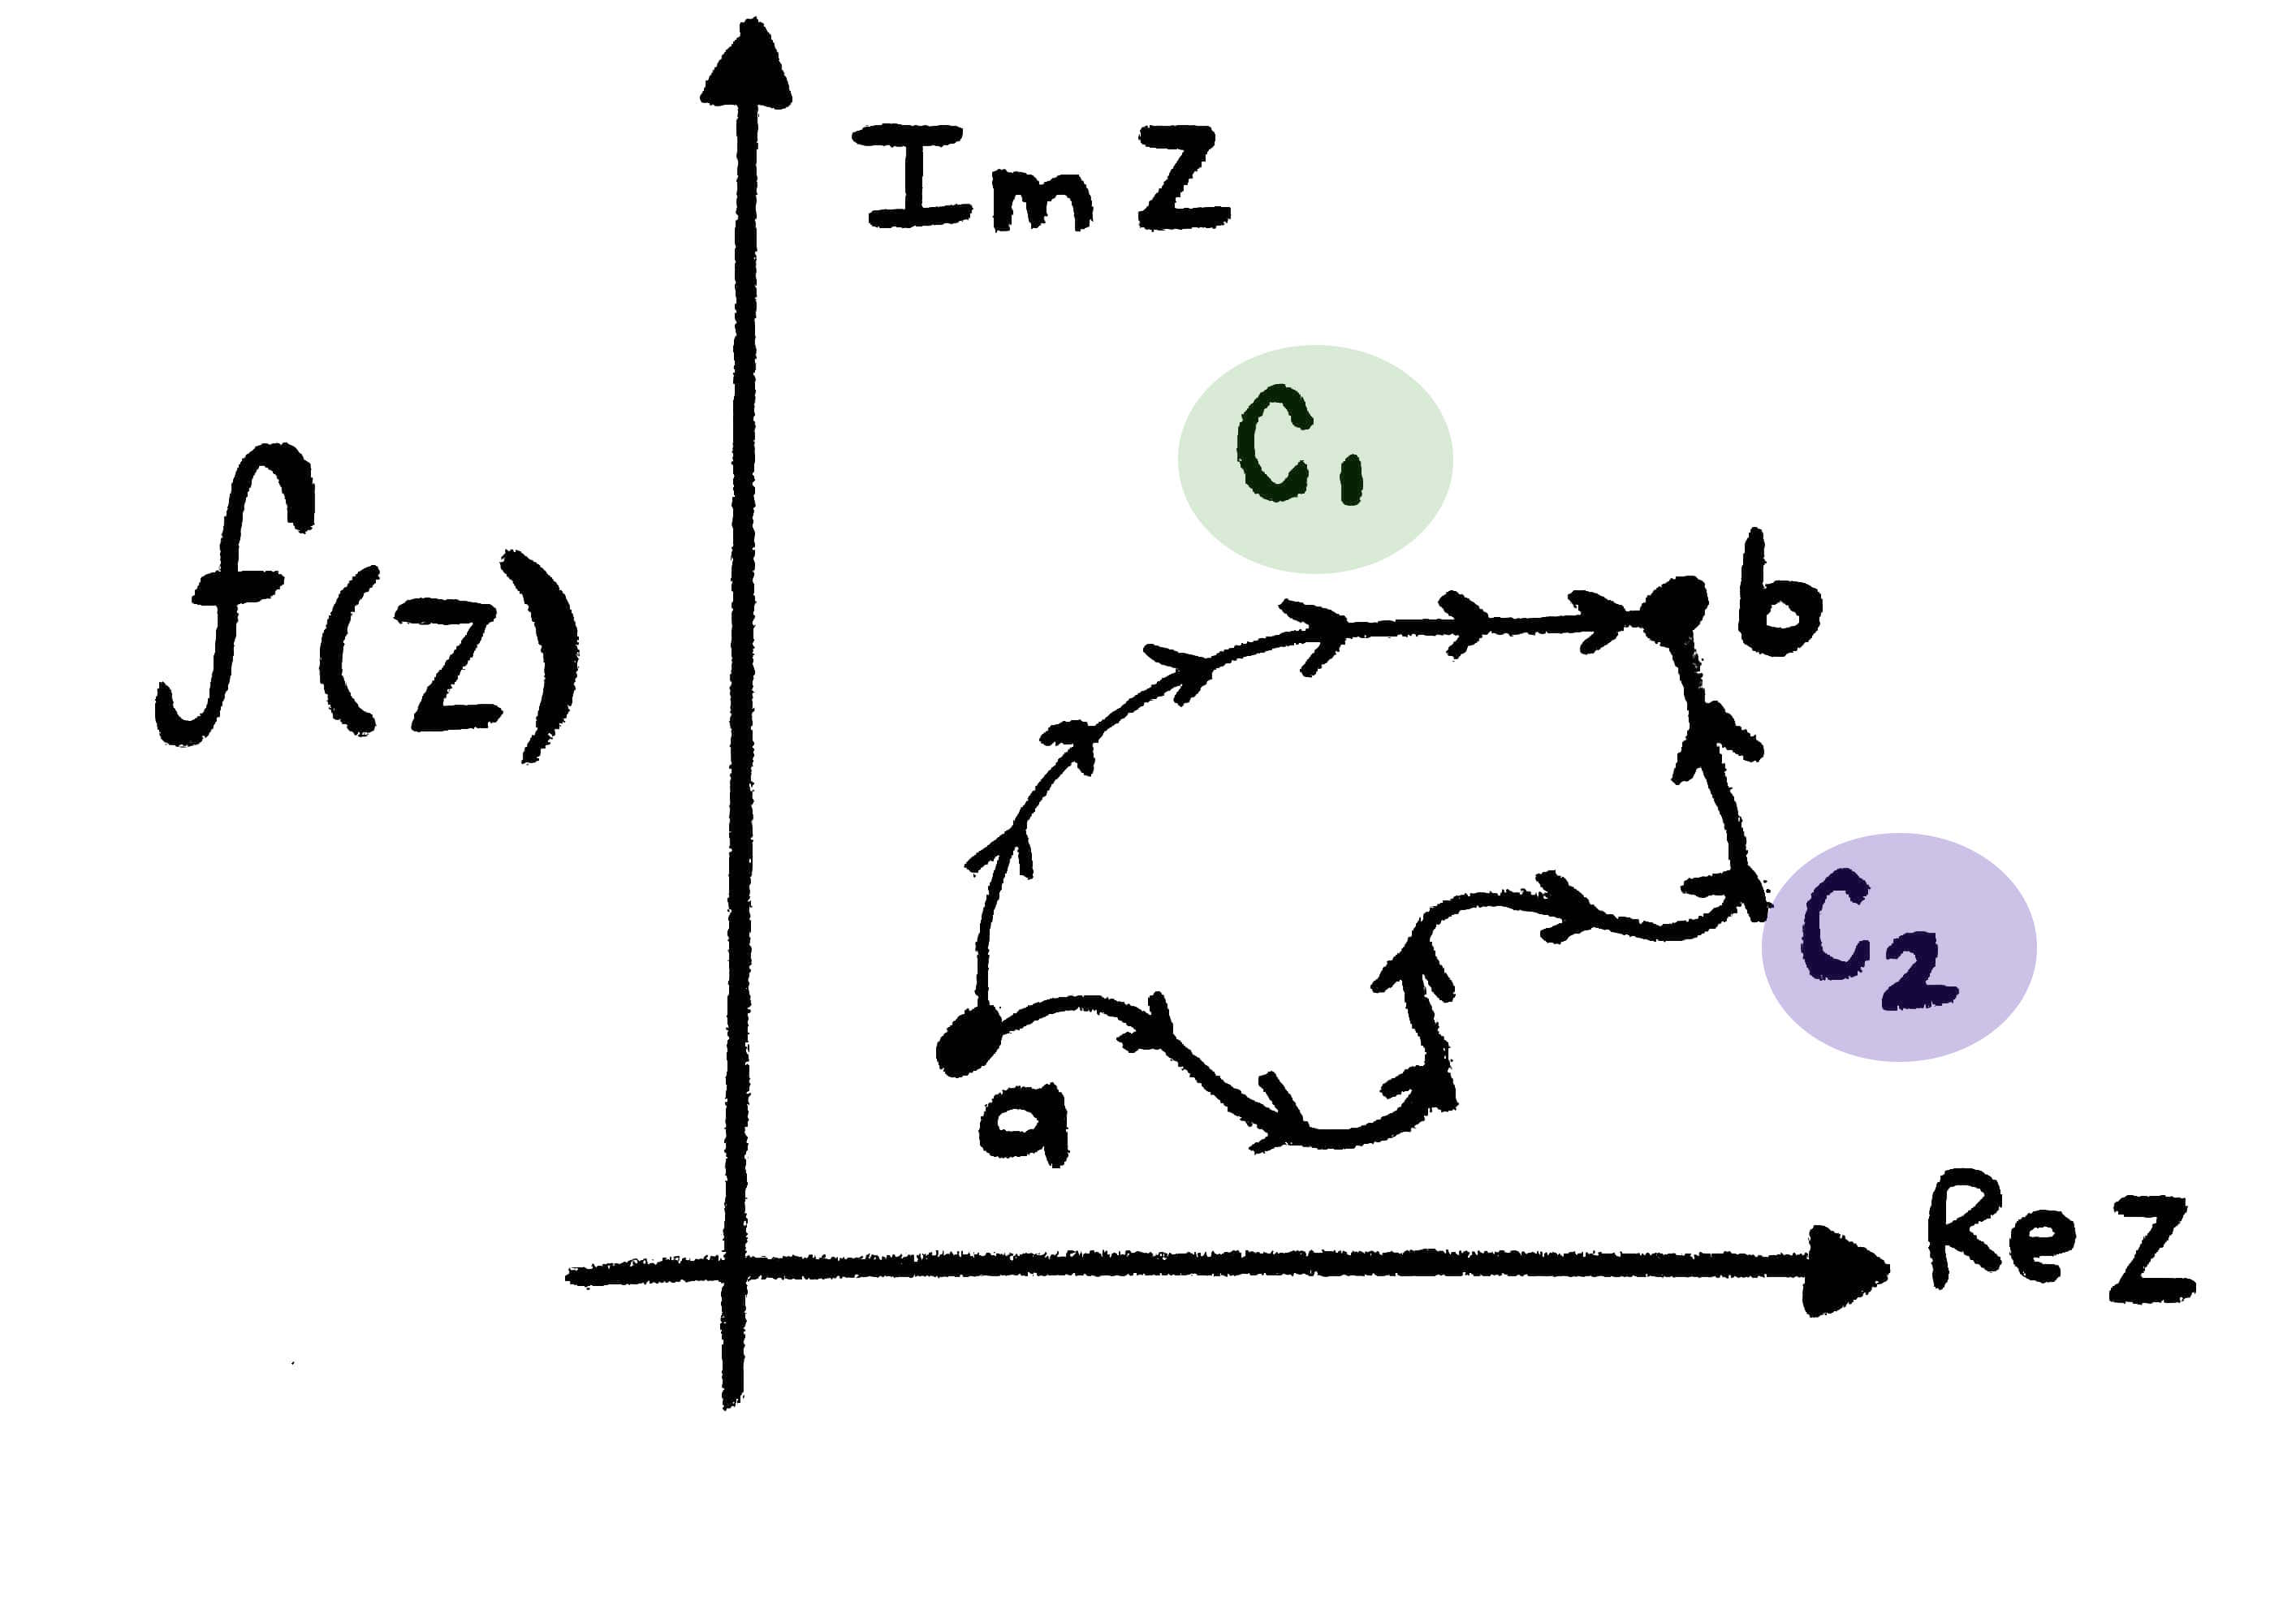
\includegraphics[width=0.43\textwidth]{CaminosDeIntegralCompleja.jpg}
                \caption{\scriptsize{¿Qué camino sigo? $C_1$ ó $C_2$}}
            \end{wrapfigure}

            Y el gran problema es que cada camino podría darte un valor diferente
            al momento de calcular la integral.

            Así que para integrar una función compleja es necesario que me digas
            cual será la curva por la cual integraremos dicha función, debido a esto
            hay grandes relaciones sobre como funciona una integral compleja y una 
            integral de línea.

            Esto se debe basicamente a que los números complejos no viven en una línea, 
            una recta númerica, sino en todo un plano complejo.


            % ==============================================
            % ========          INTEGRALES         =========
            % ==============================================
            \clearpage
            \subsection{Calcular un Integral Compleja sobre $C$}


                Supongamos que tenemos una función $f(z) = u_{(x,y)} + iv_{(x,y)}$
                sobre una curva arbitraria $\mathcal{C}$ desde el punto $a$ hasta $b$

                Supongamos que dicha curva se puede expresar usando ecuaciones parametricas
                de tal manera que $x,y$ son funciones de un párametro $t$ tal que
                así: $x(t)$ y $y(t)$.

                Entonces tenemos que podemos expresar a $a$ y a $b$ como:
                \begin{itemize}
                    \item $a = x(\alpha) + iy(\alpha)$
                    \item $b = x(\beta) + iy(\beta)$
                \end{itemize}

                Entonces ya podemos definir lo que significa una integral compleja:

                \begin{MultiLineEquation*}{3}
                    \int_C f(z) dz
                    &   = \int_C f(x+iy) (dx+idy)
                    \\& = \int_C (u +iv) (dx+idy)
                    \\& = \int_C udx - vdy + i\int_c vdx + udy 
                \end{MultiLineEquation*}

                Apliquemos un cambio de variable: 
                $dx = \frac{dx}{dt} dt$ y $dy = \frac{dy}{dt} dt$

                Por lo tanto finalmento podemos decir que:
                \begin{MultiLineEquation*}{3}
                    \int_c f(z) dz 
                        &=
                        \int_\alpha^\beta u\frac{dx}{dt} dt - v\frac{dy}{dt} dt
                        + 
                        i\int_\alpha^\beta v\frac{dx}{dt} dt + u\frac{dy}{dt} dt
                    \\  &=
                        \int_\alpha^\beta u_{(x,y)} x'(t) dt - v_{(x,y)} y'(t) dt
                        + 
                        i\int_\alpha^\beta v_{(x,y)} x'(t) dt + u_{(x,y)} y'(t) dt
                \end{MultiLineEquation*}
                


            % ==============================================
            % ========     PARAMETRIZACION         =========
            % ==============================================
            \clearpage
            \subsection{Parametrización}

                Otra forma complemente igual de valida es no parametrizar las funciones
                en parte real e imaginaria.

                Entonces podemos defininir $\int_c f(z)dz$ para cualquier curva
                cerrada. Si $C$ esta parametrizada por $r(t), \; a \leq t \leq b$
                tenemos que podemos ver a $r'(t)$ como una curva compleja y:
                \begin{equation*}
                    \int_C f(z) dz = \int_a^b f(r(t)) \; r'(t) \; dt
                \end{equation*}

                O también es común ponerlo como:
                \begin{equation*}
                    \int_C f(z) dz = \int_a^b f(z(t)) \; z'(t) \; dt
                \end{equation*}


        % ==============================================
        % ==  TEOREMA DE CAUCHY DE LAS INTEGRALES   ====
        % ==============================================
        \section{Integrales Bonitas: Antiderivadas}

            Ya que hemos aprendido todo esto sobre las integrales podemos ver que el hecho
            de parametrizar simplifica enormemente todo el trabajo que tenemos que hacer sobre
            las mismas, llegando a esto tan bonito:

            Sea $z(t) = x(t) + iy(t)$ entonces suponiendo que sean continuas en $[a,b]$
            tenemos que:
            \begin{equation*}
                \int_a^b z(t) dt 
                    = \int_a^b (x(t) + iy(t))dt
                    = \int_a^b x(t)dt + i\int_a^b y(t)dt
            \end{equation*}



        % ==============================================
        % =====  TEOREMA DE LA DEFORMACION     =========
        % ==============================================
        \section{Teorema de la Deformación}

            Sea $\Gamma$ y $\gamma$ dos trayectorias cerradas en una región del plano $R$
            con $\gamma$ en el interior de $\Gamma$.

            Sea $f(z)$ una función diferenciable en un conjunto abierta que contiene ambas
            trayectorias y todos los puntos entre ellas, entonces:
            \begin{equation*}
                \oint_\Gamma f(z) dz = \oint_\gamma f(z) dz
            \end{equation*}




        % ==============================================
        % ==  TEOREMA DE CAUCHY DE LAS INTEGRALES   ====
        % ==============================================
        \clearpage
        \section{Teorema de Cauchy}

            Si $f(z)$ es analítica y estamos hablando de una curva simple, es decir
            en la que no se cruza consigo mismo, entonces tenemos que:
            \begin{equation*}
                \oint_C f(z) dz = 0
            \end{equation*}

            % ======== DEMOSTRACION ========
            \begin{SmallIndentation}[1em]
                \textbf{Ideas}:
                
                Antes que hablar de la demostración del Teorema tenemos que recordar lo que 
                significa que una Región $R$ sea simplemente conexa.

                \Quote{Un Región $R$ es simplemente conexa si cada curva simple en $R$ es la
                frontera de una región contenida en $R$}

                De esto podemos ver que por ejemplo el disco $\Set{z \in \Complexs, \Such |z| < 1}$
                es simplemente conexo, pero el anillo $\Set{z \in \Complexs, \Such 1 < |z| < 1}$
                no lo es.


                \textbf{\\Usando el Teorema de Green}:

                Supongamos que $C$ es un curva simple cerrada que esta limitada por D
                entonces si queremos aplicar el Teorema de Green a la integral:
                $\int_C f(z) dz$ ya que tenemos que:
                \begin{MultiLineEquation*}{3}
                    f(z) dz 
                        &= (u+iv)(dx+idy)
                        &= (udx - vdy) + i (vdx + udy) 
                \end{MultiLineEquation*}
                
                Entonces podemos ver que:
                \begin{MultiLineEquation*}{3}
                    \int_C f(z) dz 
                        &=    \iint_D \Wrap{ - \Partial{v}{x} - \Partial{u}{y}} dA
                            +i\iint_D \Wrap{\Partial{u}{x} - \Partial{v}{y}} dA
                \end{MultiLineEquation*}

                Entonces el integrando será siempre cero si y solo si las ecuaciones
                de Cauchy Riemann se mantienen.
                    
            \end{SmallIndentation}
                





        % ==============================================
        % ==  TEOREMA DE LA INTEGRAL DE CAUCHY      ====
        % ==============================================
        \clearpage
        \section{Teorema de la Integral de Cauchy}

            Sea $f(z)$ analítica en el interior y sobre la frontera de $\mathcal{C}$, donde
            $\mathcal{C}$ es cerrada y simplemente conexa en una región $R$, entonces
            tenemos si $a$ pertenece a la región $R$ se cumple que:
            \begin{equation*}
                f(a) = \dfrac{1}{2 \pi i} \oint_C \dfrac{f(z) dz}{z-a}
            \end{equation*}

            Pero esta no es la forma en la que comunmente la usamos, sino que la usamos
            como un pequeño truco para poder calcular algunas integrales,
            esto lo escribimos entonces así:
            \begin{equation*}
                2 \pi i \; f(a) = \oint_C \dfrac{f(z) dz}{z-a}
            \end{equation*}






            % ==============================
            % ===   TEOREMA DE LA INTEGRAL = 
            % === VS FORMULA DE LA INTEGRAL=
            % ==============================
            \subsection{Teorema de Integral vs Formula de la Integral}
            \begin{SmallIndentation}[1em]

                Consideremos un ejemplo que creo que pone todo mas claro, 
                supon la función $f(z) = z^2 + z + 1$ a lo largo de 
                el circulo unitario.

                Por lo tanto tenemos que:
                \begin{MultiLineEquation*}{3}
                    \int_C f(z) dz 
                        &= \int_0^{2\pi} (e^{2it} + e^{it} + 1) ie^{it} dt
                        &= i \int_0^{2\pi} (e^{3it} + e^{2it} + e^{it}) dt
                \end{MultiLineEquation*}

                Creo que es muy sencillo ver que esta integral será cero, porque
                el periodo de el seno y coseno es $2\pi$, por lo tanto
                al momento de evaluar todo se cancela.

                Pero por otro lado imagina:
                \begin{MultiLineEquation*}{3}
                    \int_C \dfrac{1}{z} dz 
                        &= \int_0^{2\pi} (e^{-it}) ie^{it} dt           
                        &= i \int_0^{2\pi} dt
                        &= 2 \pi i
                \end{MultiLineEquation*}

                ¿Pero porque no dio cero?

                Porque $\dfrac{1}{z}$ es analítica en la región $\Complexs - \Set{0}$
                pero vimos que esta región no es simplemente conexa, por lo tanto no
                podemos aplicar el Teorema de Cauchy.

            \end{SmallIndentation}

                
            % ==============================
            % ========  EJEMPLO   ==========
            % ==============================
            \clearpage
            \subsection{Ejemplos}

                \begin{SmallIndentation}[1em]

                    Sea la curva aquella descrita por el circulo $|z+1|=\frac{1}{2}$
                    calcule:
                    \begin{equation*}
                        \oint_C \dfrac{dz}{z^2(z+1)}
                    \end{equation*}

                    \textbf{Solución}:

                    Simplemente tenemos que darnos cuenta que el punto de indeterminación de
                    nuestra integral es $z=0$ y $z=-1$, ahora, si te das cuenta podemos poner
                    nuestra integral como:
                    \begin{equation*}
                        \oint_C \dfrac{dz}{z^2(z- (-1))}
                    \end{equation*}

                    Entonces podemos separarlo como:
                    \begin{itemize}
                        \item $f(z) = \dfrac{1}{z^2}$
                        \item $a = -1$
                        \item $f(a) = \dfrac{1}{(-1)^2} = \dfrac{1}{1} = 1$
                    \end{itemize}

                    Por lo tanto:
                    \begin{equation*}
                        \oint_C \dfrac{dz}{z^2(z+1)} = 2 \pi i \; f(a) = 2 \pi i
                    \end{equation*}

                \end{SmallIndentation}












        % ==============================================
        % ==  TEOREMA DE DERIVACION DE ORDEN SUPERIOR ==
        % ==============================================
        \clearpage
        \section{Teorema de Derivación de Orden Superior}

            Sea $f(z)$ diferenciable en un conjunto $G$ entonces $f(z)$ tiene derivadas de todos
            los ordenes en cada punto de $G$, más aún si $C$ es una trayectoria cerrada en $G$
            que encierra unicamente puntos de $G$, en particular a $z_0$ tenemos que:
            \begin{equation*}
                f^{(n)}(z_0) = \dfrac{n!}{2 \pi i} \oint_C \dfrac{f(z) dz}{(z-z_0)^{n+1}}
            \end{equation*}

            Pero esta no es la forma en la que comunmente la usamos, sino que la usamos
            como un pequeño truco para poder calcular algunas integrales,
            esto lo escribimos entonces así:
            \begin{equation*}
                \dfrac{2 \pi i}{n!}f^{(n)}(z_0) = \oint_C \dfrac{f(z) dz}{(z-z_0)^{n+1}}
            \end{equation*}
                
            % ==============================
            % ========  EJEMPLO   ==========
            % ==============================
            \subsection{Ejemplos}

                \subsection*{Ejemplo 1}
                \begin{SmallIndentation}[1em]


                    Sea la curva aquella descrita por el circulo $|z|=\frac{1}{2}$
                    calcule:
                    \begin{equation*}
                        \oint_C \dfrac{dz}{z^2(z+1)}
                    \end{equation*}

                    \textbf{Solución}:

                    Simplemente tenemos que darnos cuenta que el punto de indeterminación de
                    nuestra integral es $z=0$ y $z=-1$, ahora, si te das cuenta podemos poner
                    nuestra integral como:
                    \begin{equation*}
                        \oint_C \dfrac{dz}{z^2(z+1)}
                    \end{equation*}

                    Entonces podemos separarlo como:
                    \begin{itemize}
                        \item $n=1$
                        \item $f(z) = \dfrac{1}{z+1}$
                        \item $f'(z) = -\dfrac{1}{(z+1)^2}$
                        \item $z_0 = 0$
                        \item $f'(z_0) = -\dfrac{1}{1^2} = -1$
                    \end{itemize}

                    Por lo tanto:
                    \begin{equation*}
                        \oint_C \dfrac{dz}{z^2(z+1)} 
                            = \dfrac{2 \pi i}{n!}f^{(n)}(z_0)
                            = (2 \pi i) -1
                            = -2 \pi i
                    \end{equation*}

                \end{SmallIndentation}

                \clearpage


                \subsection*{Ejemplo 2}
                \begin{SmallIndentation}[1em]

                    Sea la curva aquella descrita por el circulo $|z|=3$
                    calcule:
                    \begin{equation*}
                        \oint_C \dfrac{dz}{z^2(z+1)}
                    \end{equation*}

                    \textbf{Solución}:

                    Ya que nuestra curva encierra a ambos puntos de indeterminación tenemos que 
                    separarla:
                    \begin{MultiLineEquation*}{3}
                        \dfrac{dz}{z^2(z+1)} &= \dfrac{Az + B}{z^2} + \dfrac{C}{z+1}     \\
                        1 &= (Az + B)(z+1) + z^2(C)                                      \\
                        1 &= Az^2 + Bz + Az + B + Cz^2
                    \end{MultiLineEquation*}

                    Por lo tanto:
                    \begin{MultiLineEquation*}{3}
                        A + C = 0
                        \Space
                        \Space
                        A + B = 0
                        \Space
                        \Space
                        B = 1
                    \end{MultiLineEquation*}

                    Es decir:
                    \begin{MultiLineEquation*}{3}
                        A = -1
                        \Space
                        \Space
                        B = 1
                        \Space
                        \Space
                        C = 1
                    \end{MultiLineEquation*}

                    Entonces podemos separarlo como:
                    \begin{MultiLineEquation*}{3}
                        \oint_C \dfrac{dz}{z^2(z+1)}
                            &= \oint_C \dfrac{Az + B}{z^2} dz + \oint_C \dfrac{C}{z+1} dz                    
                        \\  &= \oint_C \dfrac{-(z)dz}{z^2} + \oint_C \dfrac{dz}{z^2} + \oint_C \dfrac{dz}{z+1}
                        \\  &= \oint_C \dfrac{-dz}{z} + \oint_C \dfrac{dz}{z^2} + \oint_C \dfrac{dz}{z+1}
                    \end{MultiLineEquation*}
                    \clearpage

                    Ahora vamos a ir resolviendo una por una:
                    \begin{itemize}
                        \item
                            La primera se puede resolver con la Teorema de la Integral de Cauchy
                            pues tenemos que:
                            \begin{itemize}
                                \item $f(z) = -1$
                                \item $f(0) = -1$
                            \end{itemize}

                            Por lo tanto:
                            \begin{MultiLineEquation*}{3}
                                \oint_C \dfrac{-dz}{z} = 2 \pi i f(0) = -2 \pi i
                            \end{MultiLineEquation*}


                        \item
                            La segunda se puede resolver con la Teorema de Derivación Superior
                            pues tenemos que:
                            \begin{itemize}
                                \item $f(z) = 1$
                                \item $f'(z) = 0$
                            \end{itemize}

                            Por lo tanto:
                            \begin{MultiLineEquation*}{3}
                                \oint_C \dfrac{dz}{z^2} = \dfrac{2 \pi i}{n!} 0 = 0 
                            \end{MultiLineEquation*}


                        \item
                            La tercera se puede resolver con la Teorema de la Integral de Cauchy
                            pues tenemos que:
                            \begin{itemize}
                                \item $f(z) = 1$
                                \item $f(-1) = 1$
                            \end{itemize}

                            Por lo tanto:
                            \begin{MultiLineEquation*}{3}
                                \oint_C \dfrac{dz}{z+1} = 2 \pi i f(-1) = 2 \pi i
                            \end{MultiLineEquation*}
                            
                    \end{itemize}

                    Finalmente tenemos entonces que:
                    \begin{MultiLineEquation*}{5}
                        \oint_C \dfrac{dz}{z^2(z+1)}
                            &= \oint_C \dfrac{-dz}{z} &&+ \oint_C \dfrac{dz}{z^2} &&+ \oint_C \dfrac{dz}{z+1}
                        \\  &= -2 \pi i &&+ 0 &&+ 2 \pi i
                        \\  &= 0
                    \end{MultiLineEquation*}  
                \end{SmallIndentation}



% //////////////////////////////////////////////////////////////////////////////////////////////////////////
% ///////////////////////////////////        SERIES DE FURIER       ////////////////////////////////////////
% //////////////////////////////////////////////////////////////////////////////////////////////////////////
\part{Series de Furier}
\clearpage

    % ===============================================================================
    % ========================           SERIES          ============================
    % ===============================================================================
    \chapter{Series}
        \clearpage

        % ==============================================
        % ===========    TEOREMA DE TAYLOR     =========
        % ==============================================
        \clearpage
        \section{Series de Taylor}

            Sea $f(z)$ análitica en el interior de un círculo $C_0$ con centro en $z_0$
            y radio $r_0$. Entonces para cada punto $z$ en el interior de $C_0$ se tiene
            que $f(z)$ se puede escribir como:
            \begin{equation*}
                f(z) = \sum_{n=0}^\infty \dfrac{f^{(n)}(z_0)}{n!} (z-z_0)^n
            \end{equation*}

            Además para cualquier círculo en el interior de $C_0$ la serie converge
            uniformemente.



            % =========================================
            % =========    SERIES FAMOSAS     =========
            % =========================================
            \clearpage
            \section{Series más Famosas}

                \begin{MultiLineEquation*}{3}
                    e^z = \sum_{n=0}^\infty \dfrac{z^n}{n!}
                \end{MultiLineEquation*}

                \begin{MultiLineEquation*}{3}
                    sen(z) = \sum_{n=0}^\infty \dfrac{z^{2n+1}}{(2n+1)!} (-1)^n
                \end{MultiLineEquation*}

                \begin{MultiLineEquation*}{3}
                    cos(z) = \sum_{n=0}^\infty \dfrac{z^{2n}}{(2n)!} (-1)^n
                \end{MultiLineEquation*}

                \begin{MultiLineEquation*}{3}
                    \dfrac{1}{1-z} = \sum_{n=0}^\infty z^n \Space \text{si } |z| < 1 
                \end{MultiLineEquation*}

                \begin{MultiLineEquation*}{3}
                    (1-z)^n = \sum_{n=0}^\infty \binom{n}{r} z^{n-r}
                \end{MultiLineEquation*}
                    

















\end{document}
